% chapitre 3 : chargement, gestion et représentation des données {{{
\chapter{Chargement, représentation et traitement des données}\label{chapter:03:representation}
{
    \iffalse
	% Plan {{{
	\commentaire{
		\begin{enumerate}
			%% gestion images en mémoire {{{
			\item intro : chargements d'images, recherche de voisins et génération de grille. prés du problème plus en détail
			\item travaux sur le chargement d'images\begin{enumerate}
				\item formats de sortie du microscope
				\item problème de tailles $\rightarrow$ downsampling
				\item recherche de librairies
				\item comparaison (très rapide) libtiff / tinytiff
				\item gestion de mémoire~\begin{itemize}
					\item downsampling à la volée des images, sur requête utilisateur
					\item parler de structure en mémoire une fois chargé
					\item on peut avoir autant d'images que on veut en mémoire
				\end{itemize}
				\item possibles travaux : buffer circulaire pour pas tout charger d'un coup et/ou chargement en multi-threading (a garder ici ou dans travaux à venir ?)
			\end{enumerate}
			% }}}
			\item visualisation plans de coupe
			%% KPF / Texture3D {{{
			\item Très rapide : intro à pourquoi on a fait ca :\begin{itemize}
				\item C'est un travail déjà presque entièrement fait, à tester et MàJ pour publication
				\item Ca peut nous servir d'une certaine façon pour visualiser le modèle en fin de stage
			\end{itemize}
			\item Présentation de la méthode (rapide, pas le focus du rapport)~\begin{itemize}
				\item Chargement de la texture
				\item Génération de maillage tétrahédrique à partir de maillage surfacique englobant (version binaire de la grille $\rightarrow$ maillage tétra, binariser grille $\rightarrow$ dilatation, et maillage autour de ca)
				\item (Rapide) Raymarching/Bresenham pour trouver voxel, et estimer normale et couleur
				\item Note : mentionner le fait que du coup, la complexité revient à la taille du framebuffer, non de la grille
				\item Effet de bord : on peut donc charger des grilles rentrant sur GPU, les déformer afin d'avoir une grille techniquement + grande que espace mémoire GPU
			%	\item Mentionner que ca va sortir à Vis 2020 si tout va bien
			\end{itemize}
			\item Présentation des travaux effectués (plus de détails, avec difficultés mentionnées)~\begin{itemize}
				\item Mise(s) à jour du code~\begin{itemize}
					\item 'Dépoussiérage' logiciel
					\item MaJ des shaders en GLSL : passé à qqchose de plus récent pour moins de problèmes incompatibilités
					\item Changement dans la gestion de la texture (vec4f $\rightarrow$ uchar + texture)
					\item Bug fixing pour grosses grilles
				\end{itemize}
				\item Tests de la méthode en vue de publication scientifique~\begin{itemize}
					\item Tests de performances
					\item Tests effectués sur grosses grilles
					\item Tests effectués sur petites grilles avec déformation
					\item Tests effectués à plusieurs résolutions
				\end{itemize}
				\item Difficultés encontrées sur le projet~\begin{itemize}
					\item Problème rencontré : incompatibilités Boost $\Leftrightarrow$ CGAL, et anciennes versions des libs $\Rightarrow$ problème de compilation
				\end{itemize}
			\end{itemize}
			\item Présentation des possibilités d'utilisation de la méthode dans notre cas~\begin{itemize}
				\item Une fois reconstruction effectuée, si taille grille générée $<$ taille mémoire GPU, alors possiblité de voir interactivement le modèle
				\item Générer une visu multi échelle avec fichiers comme H5F/HF5 afin de pull des infos qu'on a besoin : petit modèle sur GPU, et charger hiérarchiquement en zoomant progressivement
			\end{itemize}
			% }}}
		\end{enumerate}
	}
	% }}}
	\fi

	% Prélude : présentation chapitre {{{
	Comme vu dans le chapitre précédent, les chercheurs de l'équipe de bio-ingénierie de l'université de Tulane proposent une méthode d'acquisition tridimensionnelle à très haute résolution. Celle-ci permet d'observer les détails fins du tissu mais pose un problème : les données issues d'une acquisition sont très souvent massives, donc difficiles à manipuler et à visualiser. La première partie de ce chapitre sera consacrée aux travaux réalisés sur la gestion de mémoire lors du traitement des informations. Nous présenterons deux techniques permettant l'exploration ainsi que la visualisation en temps réel de ces données.
	% }}}
	
	% Partie chargement données {{{
	\section{Chargement d'images}\label{section:loading}
	{
        Tout d'abord vient la problématique du chargement des images en mémoire. Les coupes issues d'une acquisition sont enregistrées au format \texttt{TIF}. Nous souhaitons que notre programme soit compatible avec ce format car celui-ci est familier pour nos utilisateurs. De plus, ce format est extrêmement flexible car il permet naturellement l'utilisation de plusieurs espaces couleurs, plusieurs types de compression d'image ou même la possibilité d'utiliser une représentation multi-échelle d'une image ce qui pourra nous être utile par la suite (voir la spécification complète \href{https://www.adobe.io/content/dam/udp/en/open/standards/tiff/TIFF6.pdf}{ici} sur le site d'Adobe). 
        
        Nous avons exploré différentes pistes pour optimiser le chargement de ces données, notamment les bibliothèques \texttt{libTIFF} et \texttt{TinyTIFF}\footnote{\url{https://github.com/jkriege2/TinyTIFF}}. La première est plus générique et offre un plus grand nombre de fonctionnalités (ex : possibilité de chargement de fichier de type \texttt{BigTIFF}\footnote{Extension du format TIFF, permettant le chargement et la sauvegarde de fichiers de plus de 4Go}. La seconde est plus légère et permet de charger nos images jusqu'à 500 fois plus rapidement que \texttt{libTIFF}. Ainsi, nous avons privilégié la librairie \texttt{TinyTIFF} car notre priorité actuelle est de réduire le temps d'exploitation des données. 
        
        %les fichiers générés par le microscope utilisent peu des fonctionnalités offertes par le format, nous pouvons donc1 utiliser une bibliothèque plus simple d'utilisation permettant de lire les fichiers générés à Tulane. \`A ces fins, nous avons choisi la bibliothèque \texttt{TinyTIFF}\footnote{\url{https://github.com/jkriege2/TinyTIFF}} : elle permet de charger efficacement les fichiers \texttt{TIFF} sous plusieurs formats de données différents.
        %Malgré le fait que cette bibliothèque ne puisse pas charger les fichiers de type \texttt{BigTIFF}\footnote{Extension du format TIFF, permettant le chargement et la sauvegarde de fichiers de plus de 4Go}, elle nous permet de charger les images que Tulane nous envoie jusqu'à environ 500 fois plus rapidement que la \texttt{libTIFF}. Celle-ci fut considérée en début de projet, mais fut rejetée car même si elle permet de charger tout type de fichier \texttt{TIFF}, sa généricité rajoute de la complexité dans le code nécessaire pour la lecture complète d'un fichier, mais également plus de latence dans la lecture de fichiers.

        Nous avons également implémenté un chargeur d'images au format \texttt{DIM/IMA}, un format créé par \textit{BrainVISA} pour représenter des grilles de voxels en mémoire. Nous avons choisi ce type de fichier pour sa simplicité : un fichier \texttt{DIM} contenant les dimensions de la grille tridimensionnelle et le type des données (entiers, flottants \ldots), et un fichier \texttt{IMA} contenant les données brutes. Cette représentation nous permet d'étendre efficacement nos algorithmes de traitement de données en mode  \textit{out-of-core}\footnote{Algorithmes ne nécessitant pas de charger pas le fichier en mémoire vive pour le traiter.}. En effet, la disposition des données dans le fichier est connu, nous pouvons ainsi accéder uniquement aux données nécessaires directement sur le disque dur. Ainsi, il est possible de faire une reconstruction entière de l'échantillon sans charger l'image complète en mémoire. Cette propriété nous permet de faire passer à l'échelle les méthodes de traitement et visualisation que nous proposons et de s'assurer ainsi qu'elles soient utilisables sur les jeux de données générés par le microscope.

        Plus d'informations sur l'implémentation du chargement d'image en mémoire seront disponibles en section \ref{section:implementation}. Les images 3D chargées sont représentées par des grilles de voxels décrites dans la section suivante.
	}
	% }}}

    % Section volume {{{
	\section{Représentation des données}\label{section:voxelgrid}
	{
		À long terme, le but du projet dans lequel ce stage s'inscrit vise à analyser la morphologie ainsi que la topologie des glandes de la prostate d'un patient. Il nous est ainsi nécessaire de pouvoir représenter ces structures complexes en trois dimensions d'en étudier leur forme, et leur répartition dans l'échantillon capturé. Pour atteindre notre but, il nous faudra donc choisir une représentation tridimensionnelle économe en mémoire, permettant un parcours rapide de l'espace, préservant la topologie de l'acquisition et permettant un re-échantillonnage facile. Cette représentation des données doit aussi permettre la visualisation en temps réel des images 3D issues du microscope.

		%Il existe plusieurs façons de représenter une information spatiale tridimensionnelle. Par exemple, une suite ordonnée d'images est une première forme naïve de reconstruction tridimensionnelle, mais ne possède aucune des propriétés énoncées ci-dessus qui sont nécessaires à une analyse topologique ou morphologique. En effet, une telle suite ne possède aucune information de position absolue des images, de position relatives entre elles, ou bien de résolution spatiale des images la composant. De ce fait, il est donc impossible d'analyser la topologie de structures représentée par cette représentation des données. Explorons quelques options à notre disposition qui permettront de répondre à nos besoins.

		Il est tout d'abord important de rappeler que l'information est discrétisée, comme décrit en sections \ref{section:contexte} et \ref{section:dataset}. Ainsi, nous ne travaillons pas avec un signal continu, mais une série d'observations d'une discrétisation de ce signal. La structure de données choisie doit être capable de stocker l'information de cette acquisition afin de représenter ce signal discrétisé.

		Dans notre cas, nous avons un ensemble d'images ordonnées, avec comme informations supplémentaires la résolution spatiale des images, l'angle de capture de celles-ci, ainsi que la distance entre deux prises de vues. À partir de ces données en entrée, nous devons générer une représentation tridimensionnelle permettant une analyse topologique et morphologique de cet échantillon. Intéressons-nous donc aux approches de reconstruction volumique d'un échantillon. Il existe des structures de stockage volumiques hiérarchiques, utilisant l'espace efficacement afin de mieux représenter un ensemble de points avec un budget mémoire serré.

		L'une de ces représentations hiérarchiques d'un volume est l'\textit{octree}~\cite{cite_octree}. Cette représentation découpe une boîte englobante en 8 sous-régions de volume égaux récursivement, afin de représenter l'espace sous forme arborescente. Cette structure de données permet une bonne représentation de la répartition des données tridimensionnelles dans un espace, mais dû à sa structure arborescente ne permet pas un accès rapide aux données voisines à un point $P$ donné, ou demande une coûteuse opération de prétraitement de l'espace~\cite{cite_octree_neighbor_search} qui doit être réalisée à chaque mise à jour des données.

		Une autre solution pour stocker l'acquisition de façon volumique est le \textit{kd-tree}~\cite{cite_kd_tree}, une autre structure arborescente permettant une partition plus efficace de l'espace que l'octree. Cette structure, basée sur un arbre binaire permet de représenter un espace à $k$ dimensions, où chaque noeud non-feuille est un hyperplan\definition{Sous-espace dont la dimension est $d-1$, $d$ étant la dimension de l'espace dans lequel il existe} dans l'espace à $k$ dimensions, et où chaque noeud feuille est un point dans ce même espace. Cette structure de données permet une séparation très précise de l'espace, généralisée à $k$ dimensions. Toutefois, cette structure permet de chercher les points les plus proches à un point donné grâce à un algorithme de complexité $O(\log{n})$. Bien que cette représentation soit plus efficace que l'\textit{octree} pour le partitionnement de l'espace, cette structure abstrait toute topologie de l'espace en effectuant un partitionnement complet de celui-ci, sur les points le composant. Elle n'est donc pas adaptée à une analyse topologique ou morphologique par la suite. De plus, dans notre cas le kd-tree posséderait autant de noeuds feuille que de voxels, en possédant une structure arborescente à stocker en plus dans un budget mémoire déjà serré.

		Il existe une autre représentation qui préserve la topologie d'un signal discrétisé, possède un temps d'accès aux données constant et une recherche de voisinage en temps constant : la grille de voxels. C'est cette représentation qui est actuellement utilisée par Tulane pour stocker les acquisitions.

		% Grilles voxels {{{
		\subsection{Grilles de voxels}
		{
			Une grille de voxels, aussi appelée grille volumique, est une représentation tridimensionnelle d'un signal spatial \emph{discrétisé}. Elle est la représentation \emph{discrète} d'une fonction implicite tridimensionnelle continue attribuant une valeur, que ce soit une couleur, une température, ou une quelconque autre propriété à chaque point de l'espace. Chacun des éléments de la grille sont appelés voxels, pour \textit{\textbf{Vo}}\textit{lumetric} \textit{\textbf{El}}\textit{ement}, de la même façon que un élément d'une image est appelé pixel, pour \textit{\textbf{Pi}}\textit{cture} \textbf{\textit{El}}\textit{ement}.

			\begin{figure}[h]
			    \centering
			    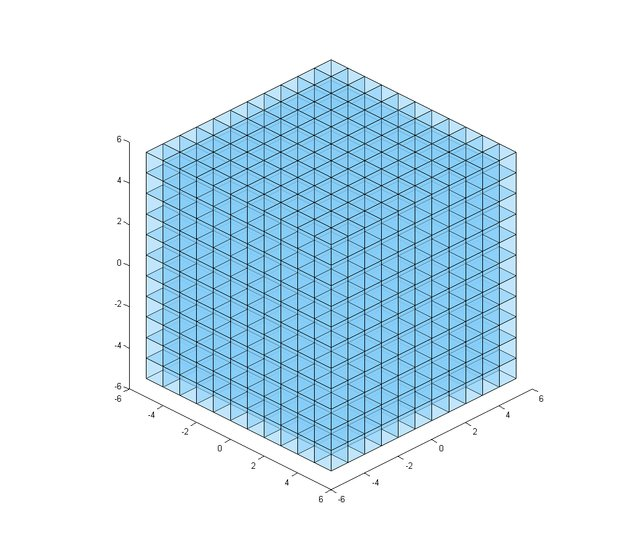
\includegraphics[width=.75\linewidth]{img/voxel_grid.jpg}
			    \captionsetup{width=.8\linewidth}
			    \caption{Une grille de voxels. On peut voir que cette grille divise l'espace régulièrement en éléments de même dimensions. Bien que cette propriété soit pratique, elle ne permet pas de réduire l'empreinte mémoire de la structure.}
			    \label{img:voxel_grid_example}
			\end{figure}

			Les grilles de voxels commencent à être utilisées dans des applications grand public depuis quelques années, dans des jeux tels que Minecraft, ou encore dans certains moteurs de rendu pour mieux représenter un milieu participatif comme un nuage de fumée~\cite{cite_voxel_smoke_rendering} par exemple. Dans le domaine médical, les grilles de voxels sont utilisées pour des acquisitions par des méthodes d'imagerie qui acquièrent un volume par coupes, comme la méthode IRM\definition{Imagerie par Résonnance Magnétique}, par exemple. En effet, il est trivial de reconstruire une grille de voxels à partir d'un ensemble de coupes d'un volume. Par exemple, le projet Visible Human\footnote{Voir \protect{\url{https://www.nlm.nih.gov/research/visible/visible_human.html}}~}~\cite{cite_visible_human} permet d'obtenir un ensemble de coupes de haute résolution d'un corps humain. À partir de ce jeu de données, nous pouvons construire une grille de voxels représentant le corps photographié.

			Il est toutefois important de noter que malgré le fait que les grilles de voxels sont ne sont pas optimisées pour partitionner efficacement l'espace. \'Etant donné que les grilles de voxels sont des grilles cartésiennes régulières, elles ne permettent pas nécessairement un stockage efficace de l'information qu'elles représentent. En effet, si le modèle que nous représentons est un modèle contenant de larges zones de vide ou des régions de matériaux uniforme, celles-ci seront représentées en haute résolution dans la grille. Une grille de voxels représente un volume englobant échantilloné régulièrement selon 3 axes et ne peut donc pas adapter la taille de ses éléments à son contenu. Pour partitionner l'espace efficacement, il nous faudrait utiliser des structures telles que des \textit{octrees} ou encore des \textit{kd-trees}. 

			Toutefois, comme vu précédemment, ces structures sont toutes deux moins adaptées à la recherche de voisins ou l'analyse topologique. L'\textit{octree} ne permet pas une recherche de voisins en temps constant, et le \textit{kd-tree} abstrait toute notion de topologie lors de sa construction.
		}
		% }}}
    }
	% }}}
	
	% Interpolation et re-échantillonage {{{
	\section{Traitement d'images tridimensionnelles}
	{
		Comme discuté en section \ref{section:voxelgrid}, les grilles de voxels sont des représentations de la discrétisation d'une fonction tridimensionnelle. Étant une représentation discrète, il nous est impossible de savoir quelle valeur est censée avoir un point contenu entre deux échantillonnages directement. Nous pouvons toutefois nous en approcher en estimant sa valeur par rapport à celle de ses voisins. Pour cela, nous utiliserons une fonction d'interpolation.

		\subsection{Interpolation}\label{subsection:interpolation}
		{
		
		    L'interpolation est une opération mathématique visant à remplacer une fonction $\mathcal{F}$ par une autre fonction $f$ coïncidant avec $\mathcal{F}$ définit en un nombre de points donnés en entrée. Cette autre fonction $f$ peut être contrainte sur plusieurs critères, notamment sur sa continuité ou discontinuité entre les points connus de la fonction d'origine $\mathcal{F}$. Il est important de distinguer l'interpolation exacte de l'interpolation inexacte. L'interpolation exacte requiert que $f$ passe par tous les points de contrôle de $\mathcal{F}$, et l'interpolation inexacte ne fait que suivre la tendance de la fonction $\mathcal{F}$ donnée par ses points de contrôle. Une comparaison visuelle est disponible en figure \ref{img:interpolation_types}.

		    \begin{figure}[!h]
		        \centering
		        \begin{subfigure}{.49\linewidth}
		            \centering
		            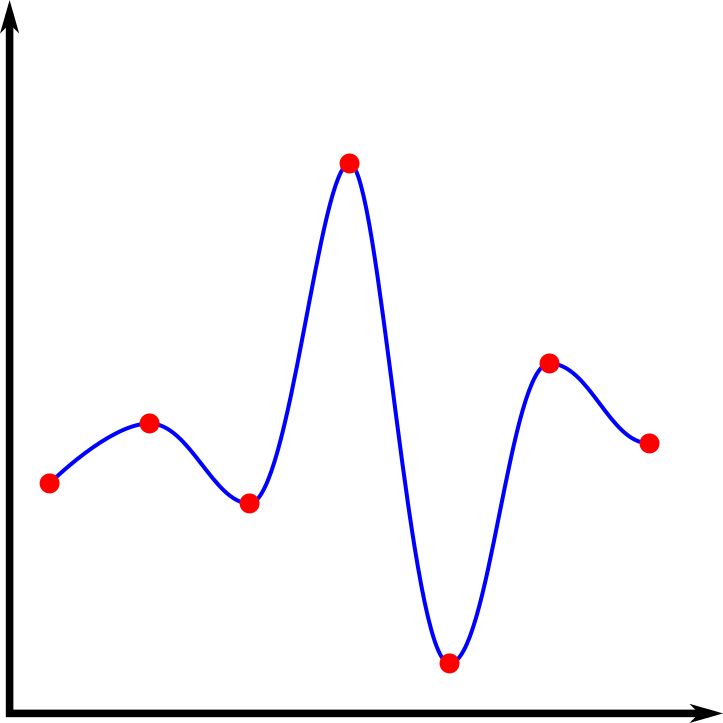
\includegraphics[width=.8\linewidth]{img/interpolation_exact.png}
		            \captionsetup{width=.8\linewidth}
		            \caption{Une fonction d'interpolation exacte, sous forme de courbe de Bézier. En rouge, les points discrétisés de la fonction $\mathcal{F}$. En bleu la courbe de Bézier $f$ passant par tous les points de $\mathcal{F}$.}
		            \label{img:interpolation_types:exact}
		        \end{subfigure}
		        \begin{subfigure}{.49\linewidth}
		            \centering
		            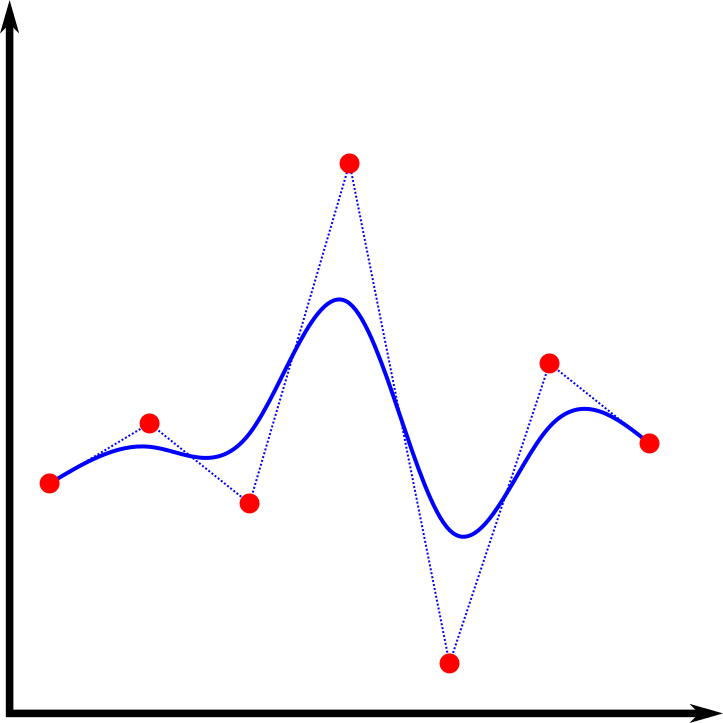
\includegraphics[width=.8\linewidth]{img/interpolation_inexact.png}
		            \captionsetup{width=.8\linewidth}
		            \caption{Une fonction d'interpolation inexacte, utilisant une B-Spline~\cite{cite_bspline_original}. En rouge, les points discrétisés de la fonction $\mathcal{F}$. En bleu pointillé, les points de contrôle de la courbe, en bleu continu la courbe finale $f$.}
		            \label{img:interpolation_types:inexact}
		        \end{subfigure}
		        \captionsetup{width=.9\linewidth}
		        \caption{Deux types d'interpolation : l'interpolation exacte (\ref{img:interpolation_types:exact}), et l'interpolation inexacte (\ref{img:interpolation_types:inexact}).}
		        \label{img:interpolation_types}
		    \end{figure}
		    
		    Grâce à l'interpolation, il nous est possible d'utiliser la fonction $f$ pour créer plus ou moins de mesures de la fonction $\mathcal{F}$, afin d'augmenter ou de diminuer la résolution de $\mathcal{F}$. Ce processus est décrit visuellement en figure \ref{img:resampling_principle}. Ainsi, nous pouvons re-échantillonner la fonction d'origine $\mathcal{F}$ grâce à une fonction $f$ choisie selon un besoin précis.

			\begin{figure}[!h]
			    \centering
			    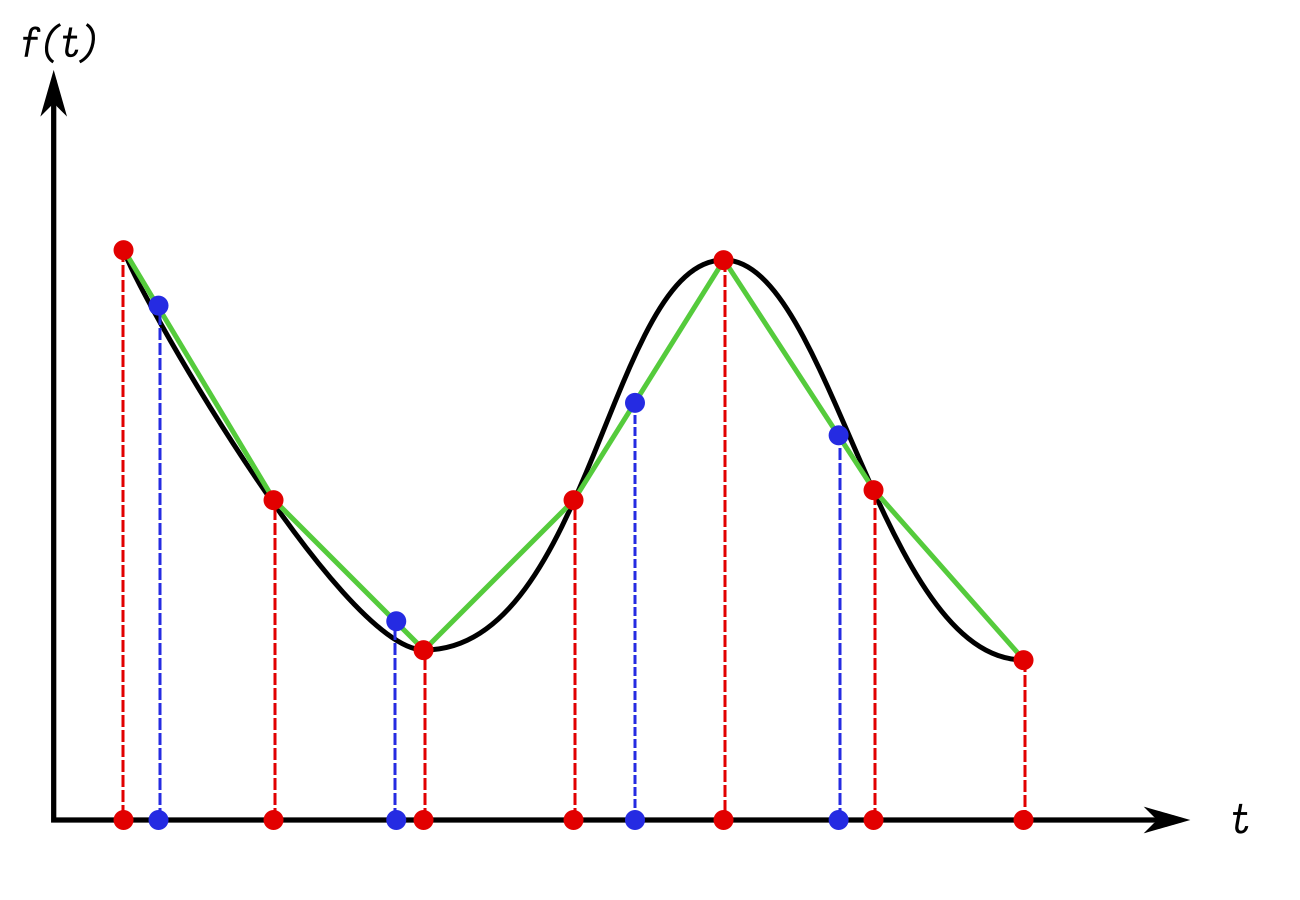
\includegraphics[width=.67\linewidth]{img/interpolation_principle.png}
			    \captionsetup{width=.8\linewidth}
			    \caption{Le principe de re-échantillonnage. En noir, le signal S avant discrétisation. En rouge, les points d'échantillonage de $S$, représentés ici sans bruit. En vert, la fonction $f$ choisie passant par tous les points échantillonnés de $S$. En bleu, les nouveaux points après l'étape de sous-échantillonnage.}
			    \label{img:resampling_principle}
			\end{figure}

		    Dans notre cas, notre fonction d'entrée $\mathcal{F}$ est une fonction bornée, représentant une acquisition bruitée d'un signal discrétisé $S$, stocké dans une grille volumique. Toutefois, dans nos travaux nous considérerons la fonction $\mathcal{F}$ comme une représentation idéale (non bruitée) de $S$, car l'annulation du bruit grâce à l'élaboration d'un modèle de bruit de l'appareil de capture \textit{di-SPIM} ne rentre pas dans le cadre de ce stage. Nous utiliserons donc des méthodes d'interpolation exactes, car la fonction $\mathcal{F}$ sera considérée comme une vérité terrain depuis laquelle nous ne voulons pas dévier.

		    Les opérations d'interpolation que nous pourrons appliquer sur $\mathcal{F}$ nous permettront de déterminer une valeur de niveau de gris pour chaque point de l'espace à l'intérieur de la grille. Ainsi, nous pourront modifier la taille de la grille localement, et proposer une méthode de re-échantillonage de la grille volumique originelle à la résolution souhaitée.

			Il existe une infinité de fonctions $f$ permettant de décrire un signal $S$ donné en entrée. Ainsi, nous allons nous réduire à uniquement quelques sous-ensembles de fonctions nous permettant d'approximer en tout point de l'espace la valeur du signal $S$ tridimensionnel donné par le microscope.

			\paragraph{Interpolation au plus proche voisin}
			{
				Cette interpolation est directement issue de la discrétisation d'un signal. Pour n'importe quel point $p$ situé entre deux échantillonnages $P_n$ et $P_{n+1}$, on attribue la valeur du point le plus proche. Cela revient à utiliser une fonction $f$ \emph{constante par morceaux}. Nous pouvons définir cette interpolation comme suit :
				\[f(p) = \left\{\begin{array}{ll} f(P_n) & \text{Si}~\frac{p-P_n}{P_{n+1}-P_n}~\leq~0.5 \\ f(P_{n+1}) & \text{Si }\frac{p-P_n}{P_{n+1}-P_n}~>~0.5 \\\end{array}\right.\]

				Vous pourrez trouver une représentation graphique de l'interpolation au plus proche voisin en figure \ref{img:interpolation_nn_with_point}.

				\begin{figure}[!h]
				    \centering
				    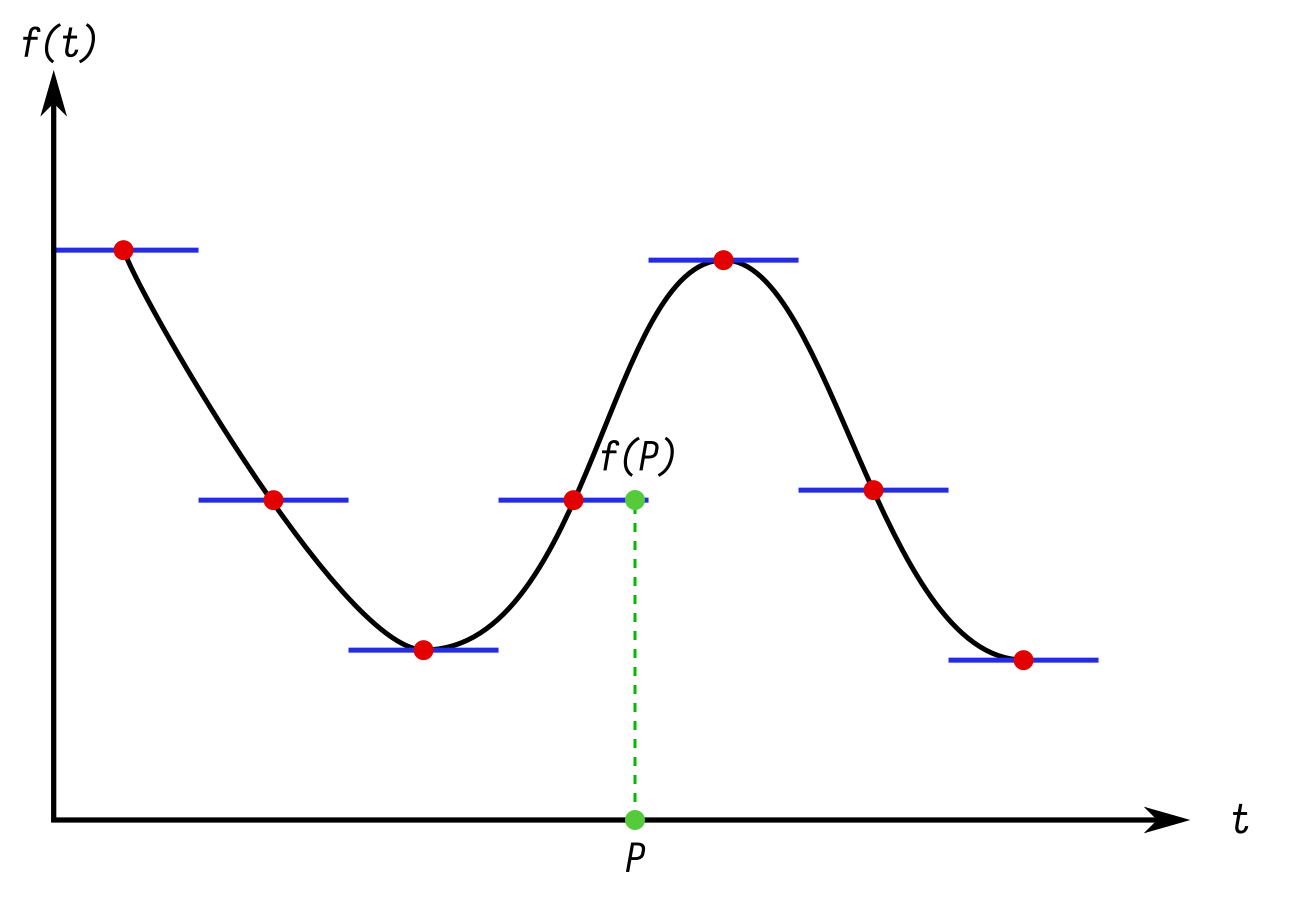
\includegraphics[width=.67\linewidth]{img/interpolation_nearest_with_point.png}
				    \captionsetup{width=.8\linewidth}
				    \caption{Une représentation graphique de l'interpolation au plus proche voisin. En noir, le signal $S$ en entrée. En bleu, la fonction $f(t)$ en tout point de l'espace borné de définition. En vert, l'estimation donnée par l'interpolation au plus proche voisin.}
				    \label{img:interpolation_nn_with_point}
				\end{figure}
				
				Il existe une variante de cette méthode d'interpolation, qui est l'interpolation au voisin le plus courant. Il suffit donc de prendre la valeur la plus courante parmi les voisins à un point $P$. Cette technique fonctionne tout aussi bien dans des images segmentées que dans des images non-segmentées.
			}

			\paragraph{Interpolation linéaire}
			{
				Cette interpolation choisit $f$ comme un ensemble de fonctions affines par morceaux. Dans ce but, on attribue à n'importe quel point $p$ situé entre deux points connus $P_n$ et $P_{n+1}$ une combinaison linéaire des deux valeurs aux points correspondant à la valeur de la courbe affine définie entre $P_n$ et $P_{n+1}$. En d'autres termes, nous avons :

				$$f(p)~=~\frac{p-P_n}{P_{n+1}-P_n}~\times~f(P_n)~+~(1~-~\frac{p-P_n}{P_{n+1}-P_n})~\times~f(P_{n+1})~~~\forall~P~\in~[P_n, P_{n+1}]$$

				\begin{figure}[!h]
				    \centering
				    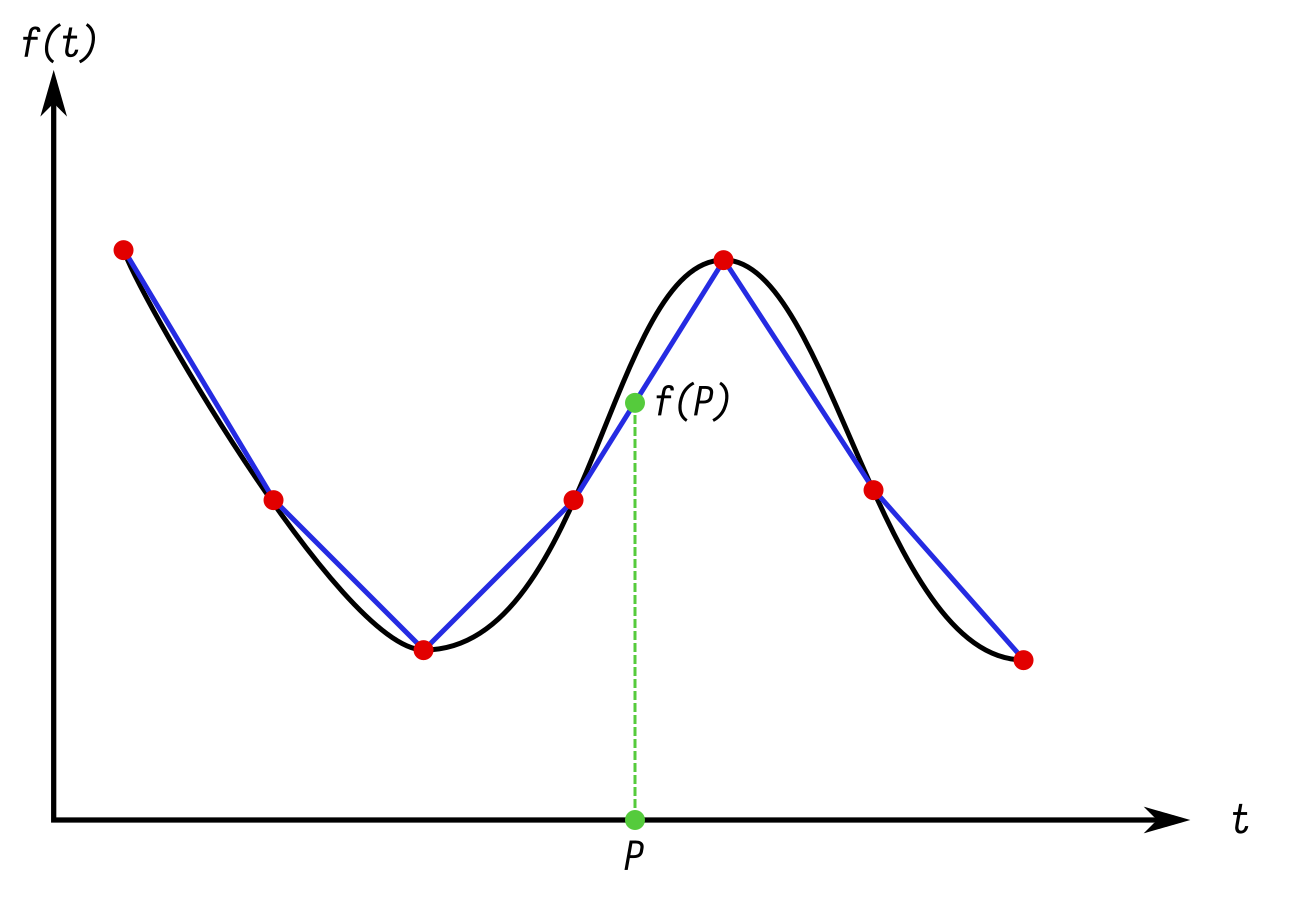
\includegraphics[width=.67\linewidth]{img/interpolation_linear_with_point.png}
				    \captionsetup{width=.8\linewidth}
				    \caption{Une représentation graphique de l'interpolation linéaire. En noir, le signal $S$ en entrée. En bleu, la fonction $f(t)$ en tout point de l'espace borné de définition. En vert, l'estimation donnée par l'interpolation linéaire.}
				    \label{img:interpolation_linear_with_point}
				\end{figure}

				Une représentation graphique est disponible en figure \ref{img:interpolation_linear_with_point}. Tout comme l'interpolation au plus proche voisin, cette méthode est définie en toutes dimensions, mais nous allons l'utiliser en 3D où elle est appelée interpolation trilinéaire. Cela signifie que nous allons interpoler trois fonctions linéaires afin de trouver la valeur de $p$. Chacune de ces fonctions sera définie sur un axe (X, Y, et Z) et permettra de faire une interpolation des valeurs aux huit points de donnée les plus proches (donc, les huit voxels les plus proches de $p$).
			}
		}
		
		\subsection{Re-échantillonnage}
		{
			Maintenant que nous pouvons interpoler une valeur en un point donné $P$ grâce aux valeurs, nous pouvons re-échantillonner le signal. Cette opération nous permet de modifier la résolution d'un signal $S$ en entrée en choisissant une fonction d'interpolation adaptée au besoin.

			Il existe deux types de re-échantillonage : le souséchantillonnage, et le suréchantillonnage. Le souséchantillonnage permet de réduire la résolution du signal en entrée, en essayant de garder autant d'information provenant du signal originel grâce à la fonction d'interpolation $f$ choisie. Le suréchantillonnage effectue l'opération inverse : il permet d'augmenter la résolution du signal, en essayant d'interpoler selon une fonction $f$ d'interpolation. Regardons l'effet sur une image, en figure \ref{img:resampling}. Nous pouvons ainsi remarquer que le type d'interpolation influe grandement sur l'image en sortie d'un re-échantillonnage. Ainsi, il est important de choisir la bonne méthode d'interpolation adaptée pour la tâche à réaliser.

			\begin{figure}[h]
			    \centering
			    \begin{subfigure}{.32\linewidth}
			        \centering
			        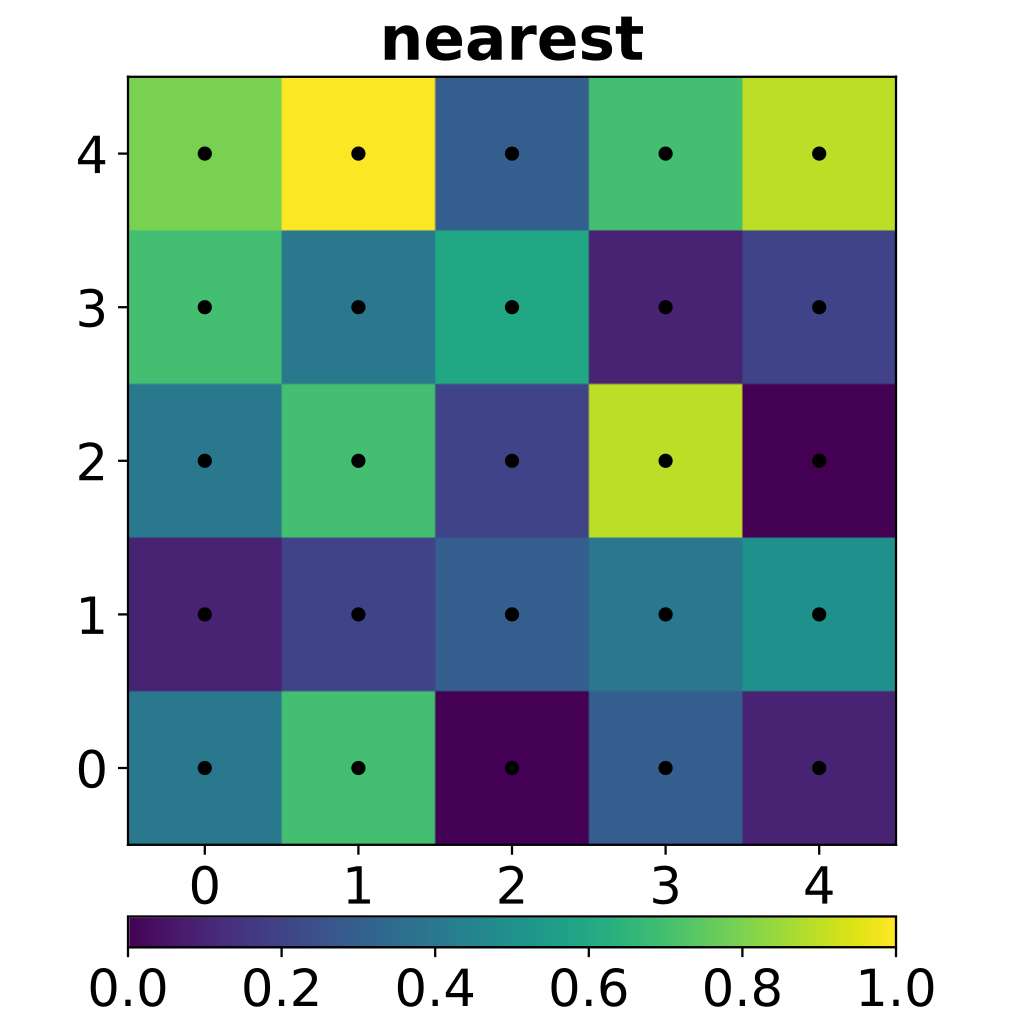
\includegraphics[width=.9\linewidth]{img/image_interpolation_nearest.png}
			        \captionsetup{width=.9\linewidth}
			        \caption{Une image interpolée grâce à l'interpolation au plus proche voisin.}
			        \label{img:resampling:nearest}
			    \end{subfigure}
			    \begin{subfigure}{.32\linewidth}
			        \centering
			        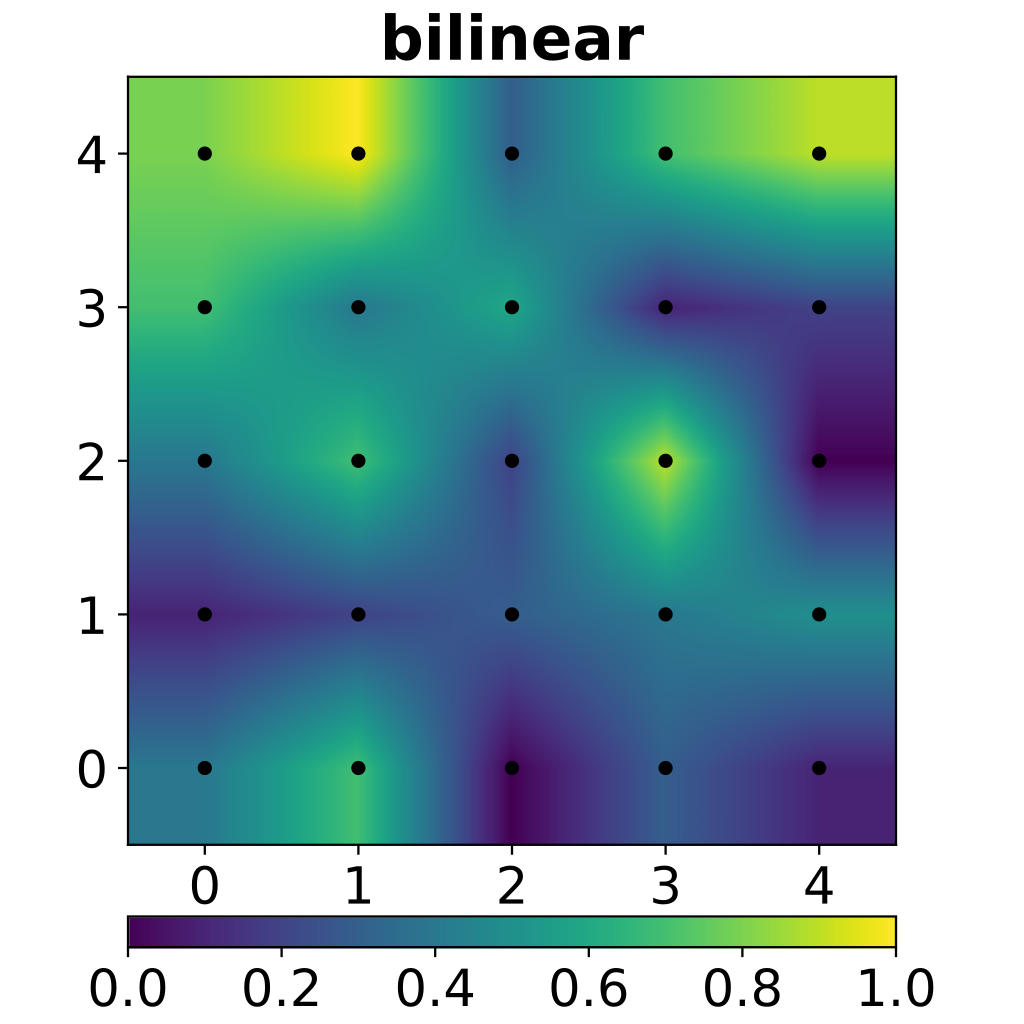
\includegraphics[width=.9\linewidth]{img/image_interpolation_bilinear.png}
			        \captionsetup{width=.9\linewidth}
			        \caption{Une image interpolée grâce à l'interpolation bilinéaire.}
			        \label{img:resampling:bilinear}
			    \end{subfigure}
			    \begin{subfigure}{.32\linewidth}
			        \centering
			        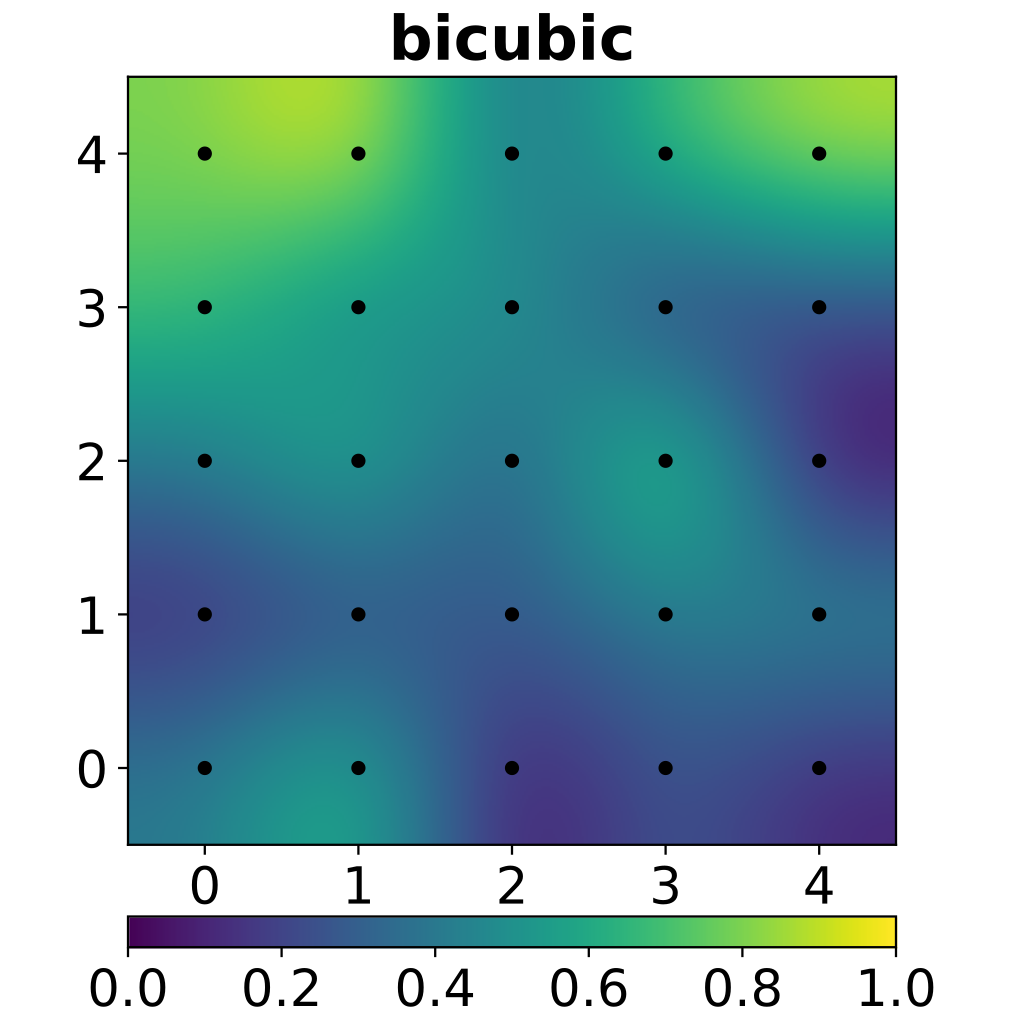
\includegraphics[width=.9\linewidth]{img/image_interpolation_bicubic.png}
			        \captionsetup{width=.9\linewidth}
			        \caption{Une image interpolée grâce à l'interpolation bicubique.}
			        \label{img:resampling:bicubic}
			    \end{subfigure}
			    \captionsetup{width=.9\linewidth}
			    \caption{Différentes méthodes d'interpolation pour une image. Copyright Zykura, Wikimedia Commons, sous licence \href{https://creativecommons.org/licenses/by-sa/4.0/deed.en}{CC-BY-SA-4.0}}
			    \label{img:resampling}
			\end{figure}

			Dans notre cas, nous allons devoir re-échantillonner les images représentant l'échantillon de prostate d'un patient. En effet, comme sera expliqué dans la section \ref{section:microscopy}, nous avons deux piles d'images prise à deux angles de vue différents pour un seul échantillon. Afin de reconstruire l'échantillon en trois dimensions, il nous faudra pouvoir accéder à des informations des piles d'image en entrée, qui peuvent ne pas être des positions où un échantillon est directement disponible. Ainsi, il nous faudra pouvoir re-échantillonner les images d'entrée à la volée, afin de pouvoir avoir une méthode de génération de grille faite en temps réel, sans pré-traitement sur les données en entrée. Ces re-échantilonnages sont également utiles pour la gestion mémoire, que nous allons voir en section suivante.
		}
	}
	% }}}

	% Partie gestion mémoire {{{
	\section{Gestion de la mémoire}\label{section:memory}
	{
		%Afin de proposer une méthode de traitement des données générées par le microscope, il faut pouvoir être capable de charger et d'analyser lesdites données. Nous avons vu dans la section \ref{section:loading}, nous pouvons charger des fichiers représentant des piles d'images en mémoire grâce à l'utilisation de bibliothèques externes.

		Nous avons proposé en section \ref{section:loading} deux méthodes de chargement d'images, et nous avons étudié en section \ref{section:voxelgrid} la représentation choisie pour représenter les images issues du microscope. Une fois ces images chargées, il nous faut les disposer en mémoire de façon efficace, afin de pouvoir charger le plus de données possibles pour la visualisation qui va être effectuée par la suite.

		\subsection{Utilisation et disposition mémoire}
		{
            %Un des objectifs de ce stage est la visualisation en temps réel du jeu de données, une première méthode simple d'exploration des données fut donc implémentée (voir section \ref{section:visualisation:cuttingplanes}). Pour que cette méthode fonctionne, l'intégrité des données à afficher doit pouvoir être contenue intégralement dans la mémoire vive du processeur graphique de l'application. À plus long terme, nous pourrons implémenter une méthode de visualisation plus complexes ne nécessitant pas de charger l'intégrité des données en mémoire.
    
            Nous proposons dans un premier temps une méthode permettant de réduire la taille des données afin de travailler sur des données rentrant entièrement en mémoire. Cela permet de proposer sur une première version des algorithmes de traitement et de visualisation sur une quantité de données plus facilement gérable et de passer à l'échelle ensuite. De plus, cela permet à l'utilisateur d'interagir avec une version basse résolution de l'image 3D, l'explorer, décider des traitements nécessaire en temps réel et d'appliquer le même processus hors-ligne aux données haute-résolution une fois qu'il est satisfait du résultat. 
            
            %Les jeux de données bruts étant trop massifs pour rentrer en mémoire, une première passe de pré-traitement des données est parfois nécessaire afin de réduire la taille des images chargées.
            Ainsi, l'utilisateur peut demander d'effectuer un sous-échantillonnage au plus proche voisin au moment de charger les images. Si nécessaire, ce re-échantillonage est donc appliqué sur l'image, chargeant une version basse résolution de celle-ci. Sur nos données, un sous-échantilonnage à $\frac{1}{4}$ de la résolution initiale nous permet de charger la quasi-intégrité de l'image 3D en mémoire, tout en gardant l'information contenue dans les captures. Si l'utilisateur ne demande pas d'effectuer cette passe, alors l'image est chargée directement en mémoire, à pleine résolution.

			%C'est à cette étape du processus qu'il est possible d'appliquer d'autres opérations de pré-traitement sur les images. Par exemple, on pourrait binariser\definition{Rendre une image en noir ou blanc selon une valeur de seuil} l'image, ou la segmenter selon plusieurs sous-domaines, ou encore la re-dimensionner de façon à ne pas avoir de zones de vide autour de la donnée.

			Une fois chargées, les données contenues dans la grille sont ordonnées dans un tableau unidimensionnel en mémoire, ligne par ligne (selon l'axe X). Ainsi, lorsque nous souhaitons évaluer la valeur d'un élément de cette grille à un point $P(x,y,z)$ défini dans l'espace de la grille, nous calculons d'abord l'indice $(i,j,k)$ correspondant à la partie entière des coordonnées de $P$ (voir figure \ref{img:voxel_fetch}). À partir de cet indice, il est trivial d'accéder à la bonne case mémoire du tableau contenant l'information à cet endroit. Grâce à cette organisation mémoire, nous pouvons avoir un accès aux données dans la grille en temps constant.

			\begin{figure}[h]
			    \centering
			    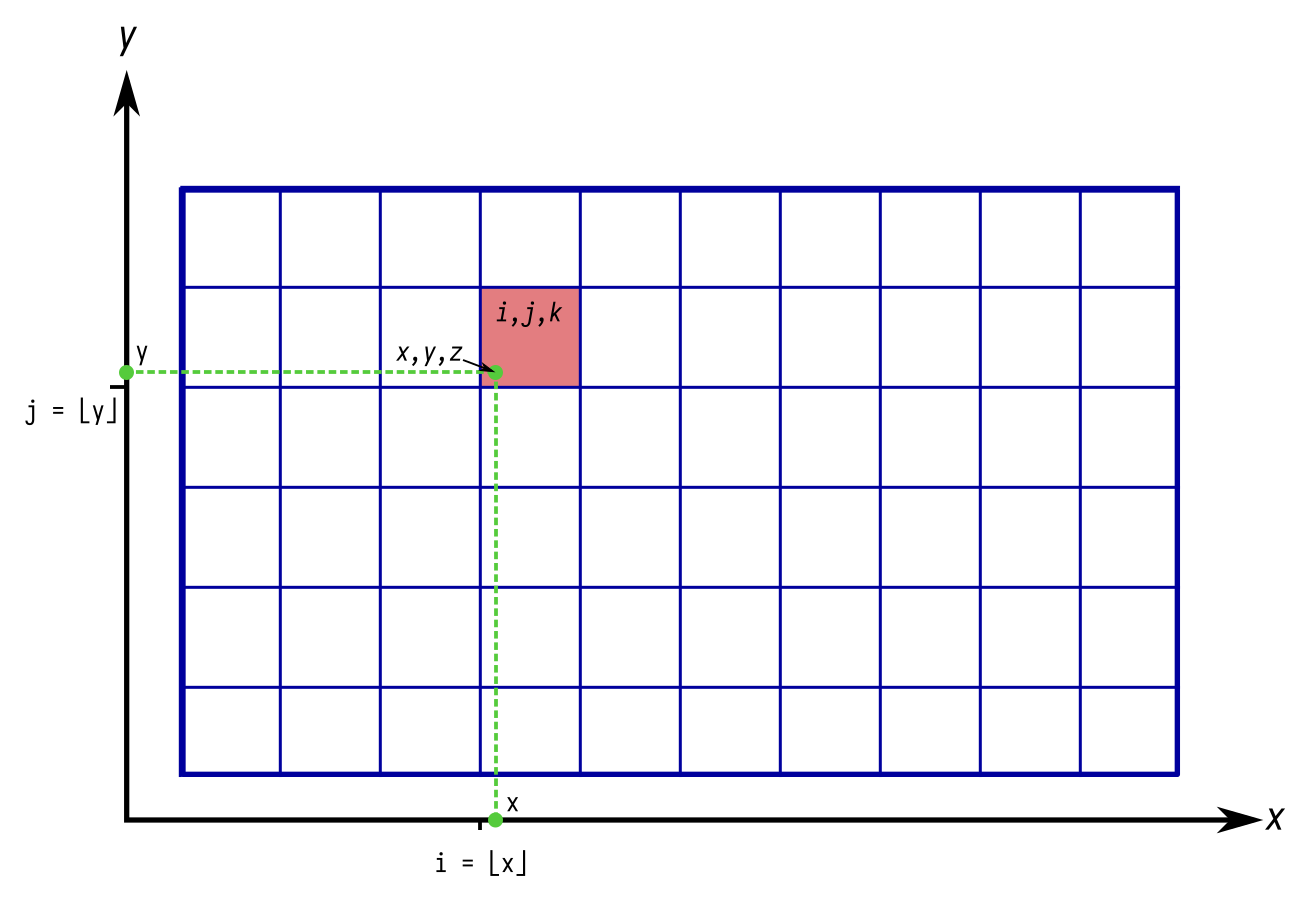
\includegraphics[width=.8\linewidth]{img/voxel_grid_fetch.png}
			    \caption{\'Evaluation de la valeur du voxel contenant le point $P(x,y,z)$}
			    \label{img:voxel_fetch}
			\end{figure}

			Cette organisation par lignes est également utilisée afin de passer les informations nécessaires au moteur de rendu pour pouvoir afficher la pile d'images à l'écran. Plus de détails seront disponibles dans la section \ref{section:implementation}.

            % À ignorer :
			%Par exemple, pour le jeu de données de l'échantillon de prostate, avec la fonction de re-échantillonnage activée, notre méthode peut stocker la grille de voxels représentant une pile d'images en utilisant seulement un quart de la mémoire nécessaire pour le stocker en taille réelle. Il est donc possible d'utiliser cette méthode afin de charger le jeu de données entier sur des ordinateurs ne possédant que 4 giga-octets de mémoire vive. Pour les ordinateurs possédant moins de mémoire vive, ou pour des jeux de données de taille bien supérieure (comme expliqué dans la section \ref{section:dataset}), un travail supplémentaire pourra être effectué afin de ne charger qu'un sous-ensemble d'images, appartenant à une zone d'intérêt pour la tâche réalisée au moment demandé ou bien en chargeant des images d'encore plus basse résolution. Pour l'instant, l'opération de re-échantillonnage est simplifiée et ne charge l'image qu'à un quart de sa résolution originelle, mais il serait par la suite possible d'adapter cette méthode de chargement afin de charger une version basse résolution adaptée à un budget mémoire maximum donné par l'utilisateur.

            % Ici : je veux dire que le downsampling n'est là que pour la visu, et que on pourrait effectuer des travaux en plus pour charger des sous parties de l'image afin de reconstruire l'échantillon (ou meme faire out of core) :
			%Cette méthode permet de charger des jeux de données à basse résolution, pour des fins de visualisation. Toutefois, si l'utilisateur souhaite reconstruire un échantillon, il est possible de ne pas effectuer cette opération de pré-traitement et de charger les données.
		 }
	}
	% }}}
}
% }}}

% Chapitre 04 : visu {{{
\chapter{Visualisation d'images 3D}\label{chapter:04:visualisation}
{
	% Interlude : présentation API graphiques {{{
	Une fois les images chargées, nous pouvons maintenant les visualiser. Nous détaillerons dans un premier temps l'environnement technique dans lequel ces méthodes furent élaborées avant de avant de détailler les méthodes de visualisation proposées. En effet, nous avons besoin de plusieurs choses afin de rendre une visualisation interactive d'un objet possible :\begin{itemize}
		\item une bibliothèque permettant la création d'interfaces graphiques,
		\item une API\definition{\textit{Application Programming Interface}} de rendu,
		\item une bibliothèque permettant de contrôler une caméra virtuelle.
	\end{itemize}

	La bibliothèque d'interface graphique nous est nécessaire afin de donner le contrôle à l'utilisateur du programme de façon simple, et rapide à comprendre. L'API de rendu doit idéalement être indépendante du matériel informatique utilisé. Et enfin, la bibliothèque de contrôle caméra servira pour l'interaction entre l'utilisateur et l'échantillon acquis.

	Pour créer l'interface, nous avons choisi la bibliothèque \textit{Qt}\footnote{\url{https://www.qt.io/}}. \textit{Qt}, développée en C++ permet de créer des exécutables d'un programme sous plusieurs plateformes. Cette API permet également de créer et de gérer des fenêtres pour que l'utilisateur puisse avoir un retour à l'écran, ainsi que des boutons et de curseurs pour interagir avec le programme. Cette bibliothèque permet aussi de mettre en places des interactions entre différents composants d'une application.
	
	Pour l'API de rendu, nous avons choisi \textit{OpenGL}\footnote{\url{https://www.khronos.org/opengl/}}. Cette API, disponible sur toutes les plateformes majeures, ne dépend pas du matériel sur lequel le programme s'exécute, et est assez simple à configurer par rapport à une API comme \textit{Vulkan}\footnote{\url{https://www.khronos.org/vulkan/}} par exemple. De plus, \textit{Qt} propose un ensemble de composants utiles à la gestion des applications utilisant \textit{OpenGL}.
	
	Enfin, pour notre méthode de contrôle de caméra, nous avons choisi la bibliothèque \textit{QGLViewer}\footnote{\url{http://libqglviewer.com/}} permettant, par sa simplicité, d'avoir très rapidement une application interactive en utilisant un environnement \textit{Qt}+\textit{OpenGL}.

	La combinaison de ces trois principaux composants nous permet de nous abstraire du système exécutant le programme, et d'assurer un fonctionnement constant sur plusieurs configurations matérielles.

	Dans la suite de ce chapitre, nous présentons des concepts présents dans l'API \textit{Qt}, ainsi que des fonctionnalités d'\textit{OpenGL}. Nous aborderons également quelques modes de rendus couramment utilisés dans le domaine de l'informatique graphique (plus d'informations en annexes). 
	%Elles contiendront une brève présentation des fonctionnalités de \textit{Qt} et plus particulièrement de son mécanisme de connexion \textit{Slot-Signal}, ainsi que plus de détails sur les différents modes de fonctionnement d'\textit{OpenGL} afin de pouvoir comprendre les opérations effectuées par la suite et leurs termes techniques associés.
	% }}}

    % etat de l'art visualisation {{{
    \section{État de l'art sur la visualisation}
    {
        Dans le milieu des images médicales, il existe un grand nombre de méthodes permettant de visualiser des données patient interactivement. Celles-ci peuvent être classées en deux grandes familles, les visualisations surfaciques ainsi que les visualisations volumiques interactives. Dans nos travaux, nous proposons une méthode d'exploration par rendu surfacique, ainsi qu'une méthode de rendu de grilles de voxels. Toutefois, nous présentons ici les principes au c\oe{}ur des techniques de visualisation d'image médicales, afin de pouvoir étudier les avantages et inconvénients de chacun d'entre eux.

        % surfaciques {{{
        \subsection{Visualisation surfacique}
        {
            Les méthodes de visualisation surfaciques d'images médicales permettent de visualiser une image tridimensionnelle grâce à l'utilisation de primitives géométriques sur lesquelles les données de l'image sont appliquées ou projetées. Les primitives géométriques utilisées pour ce type de rendu sont le plus souvent des surfaces créés en pré-traitement de la visualisation de l'image tridimensionnelle. Ces méthodes permettent de visualiser une ou plusieurs surfaces représentant les bordures/frontières des différents types de contenu présents dans l'image tridimensionnelle, sans avoir à analyser et afficher les données brutes de cette image à chaque rafraîchissement de l'écran. Par exemple les frontières entre les différents organes du patient, Figure \ref{img:vr_slicer}. Dans \textit{The Lab}, un jeu en réalité virtuelle développé par \textit{Valve Corporation}, un crâne est présenté à l'utilisateur. Celui-ci fut d'abord numérisé grâce à un appareil de tomodensitométrie, puis ensuite un maillage surfacique fut construit grâce à une méthode appelée \textit{marching cubes}~\cite{cite_marching_cubes} afin de pouvoir être affiché à l'écran. Dans cet exemple, seul l'os du crâne fut numérisé. Les couches supplémentaires semi-transparentes de muscles et de peau (en rouge et jaune respectivement sur les images) furent ajoutées manuellement par un groupe d'artistes au cours du développement du jeu. Cette représentation est bien souvent moins onéreuse en mémoire et plus rapide à afficher que l'image tridimensionnelle originelle pour de gros jeux de données, et permet également de ne traiter que les parties de l'image contenant des données considérées comme utiles.

            \begin{figure}[h]
                \centering
                \begin{subfigure}{.45\linewidth}
                    \centering
                    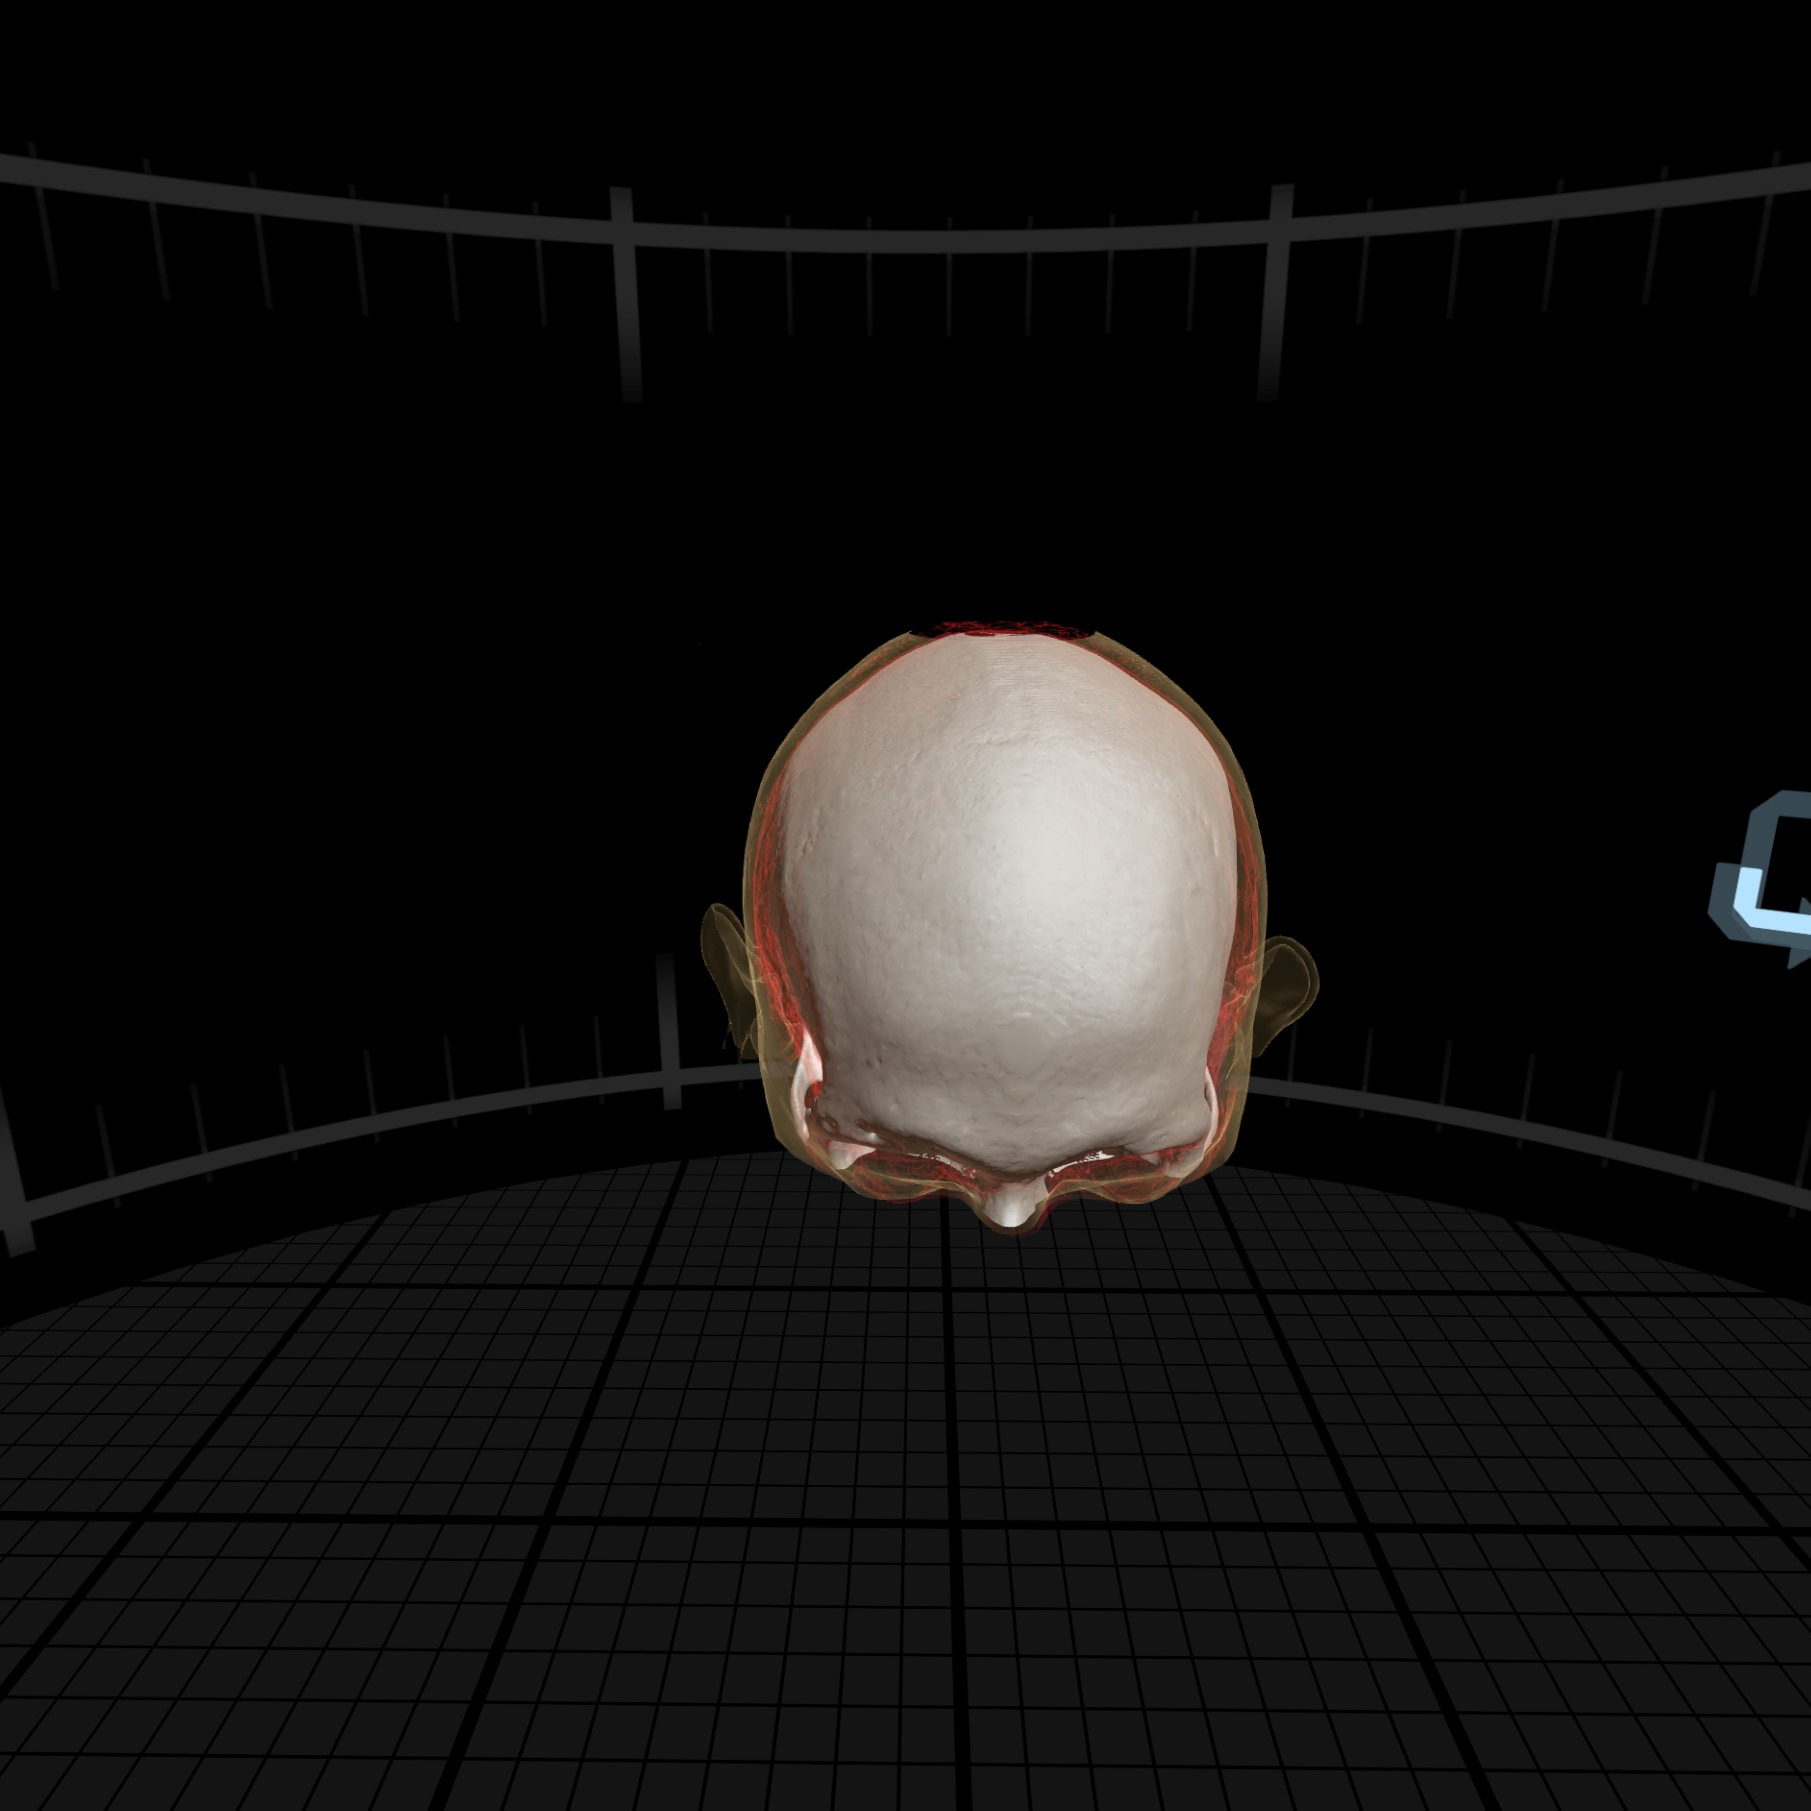
\includegraphics[width=.8\linewidth]{img/vrview_1.jpg}
                    \captionsetup{width=.8\linewidth}
                    \caption{La surface de ce crâne fut extraite d'une image médicale grâce à l'algorithme de \textit{marching cubes}.}
                    \label{img:vr_slicer:original}
                \end{subfigure}
                \centering
                \begin{subfigure}{.45\linewidth}
                    \centering
                    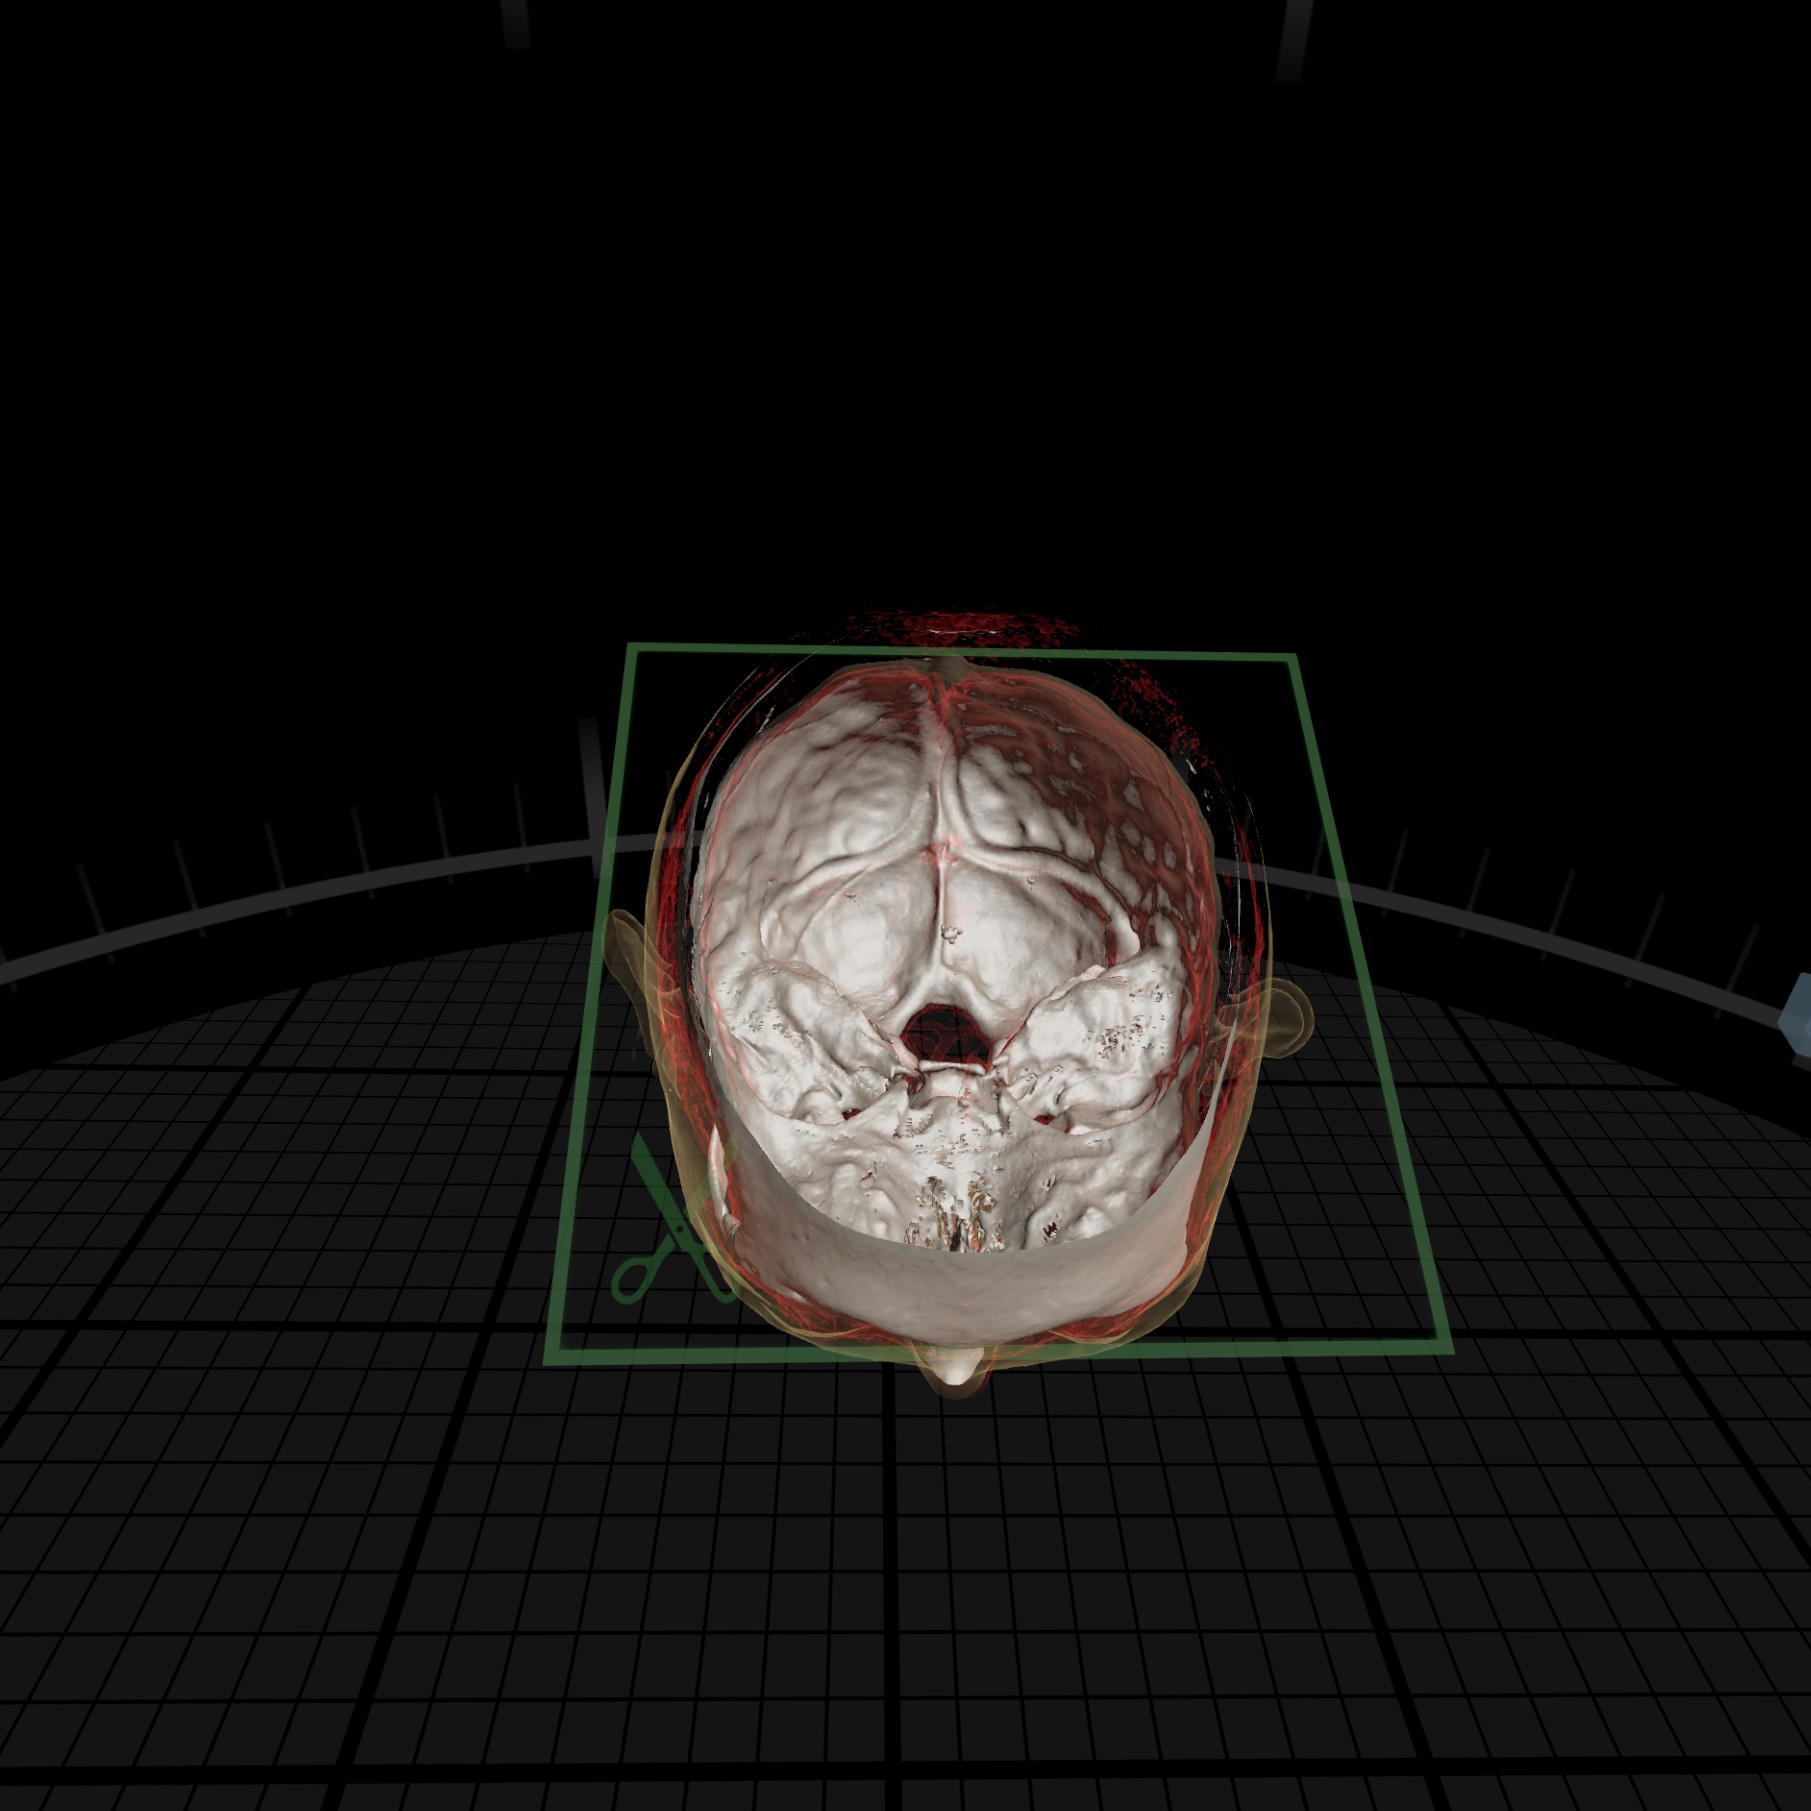
\includegraphics[width=.8\linewidth]{img/vrview_2.jpg}
                    \captionsetup{width=.8\linewidth}
                    \caption{Le plan de coupe permet de voir une sous-partie de l'isosurface extraite originellement.}
                    \label{img:vr_slicer:sliced}
                \end{subfigure}
                \caption{Application de visualisation par plans de coupe d'un maillage surfacique en réalité virtuelle. (Copyright Valve, 2016)}
                \label{img:vr_slicer}
            \end{figure}

            L'algorithme des \textit{marching cubes} est un algorithme permettant l'extraction d'une isosurface\definition{Fonction $F$ satifaisant $F(v)=\alpha$ dans un champ scalaire} depuis une image médicale tridimensionnelle. Afin d'extraire cette isosurface, il est nécessaire que l'utilisateur donne une valeur seuil $\alpha$ à partir de laquelle on considère une donnée comme \og{}significative\fg. Cet algorithme analyse tous les voxels de l'image en entrée ainsi que leur voisinnage direct, et construit une représentation surfacique en fonction de la présence ou non de données significatives dans les voxels du voisinage, comme vu en figure \ref{img:marching_cubes_configs}. Bien que cette méthode ne soit pas la première méthode d'extraction d'isosurfaces (dont le premier exemple fut une méthode par \textsc{Wyvill}~\cite{cite_wyvill_cubes}), c'est la méthode la plus utilisée dans le cadre de traitement d'images médicales tridimensionnelles~\cite{cite_marching_cubes_popularity}. Des extensions ont permis de combler quelques lacunes présentes dans le travail originel de \textsc{Lorensen} et \textsc{Cline}. Notamment, \textsc{Nielson} et \textsc{Hamman}~\cite{cite_marching_cubes_uncertainty} démontrent des ambiguïtés présentes dans la version originelle de l'algorithme, et introduisent aussi une méthode permettant d'enlever cette ambiguïté en utilisant une interpolation bilinéaire des valeurs ambiguës afin de savoir quelle configuration appliquer à un voxel donné.

            \begin{figure}[h]
                \centering
                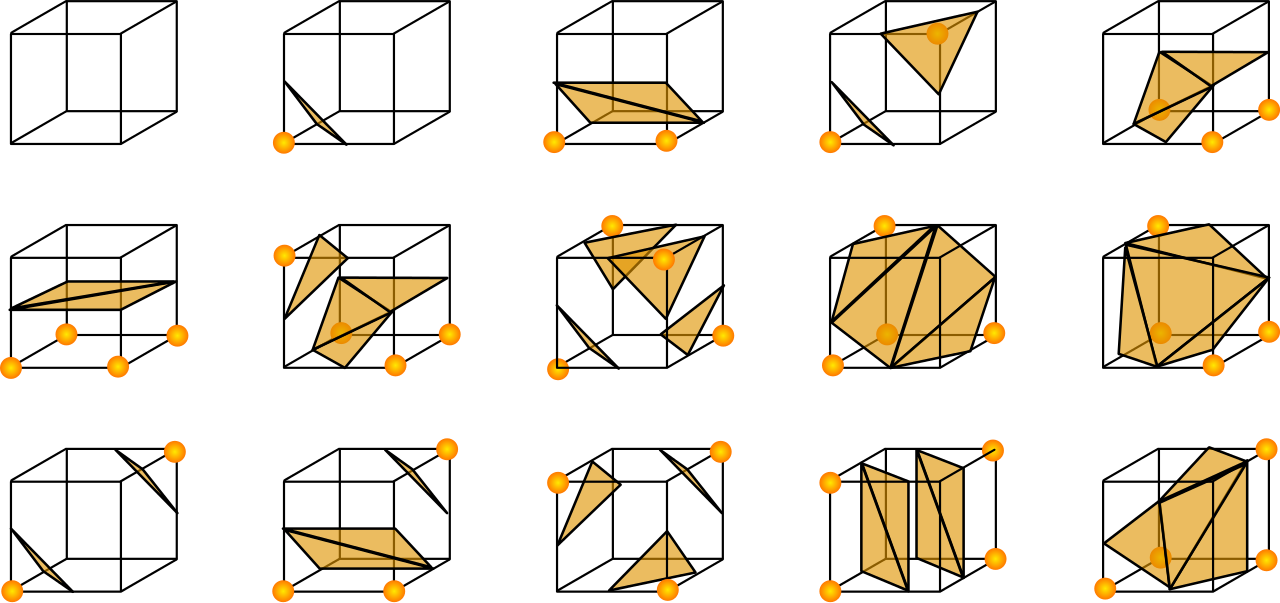
\includegraphics[width=.8\linewidth]{img/marching_cubes_topology.png}
                \captionsetup{width=.8\linewidth}
                \caption{Les 15 configurations initiales permettant de générer des surfaces grâce au voisinage d'un voxel. Les points en jaunes sont des voxels considérés comme significatifs.}
                \label{img:marching_cubes_configs}
            \end{figure}

            Ces représentations des isosurfaces présentes dans les images médicales sont extrêment pratiques pour la visualisation interactive d'un échantillon, car elles ne contiennent que peu de données (points et faces) à afficher et à traiter comparé à une image volumique de la même résolution. De plus, les cartes graphiques sont plus adaptées à faire du rendu de maillages surfaciques, car des maillages du même type sont fréquemment utilisés pour des application graphiques intensives, telles que des jeux vidéos ou des applications de CAO.

            Toutefois, l'un des principaux désavantages de ces méthodes de rendu est qu'ils n'affichent que l'isosurface extraite d'une image tridimensionnelle ou d'un sous-ensemble de valeurs de celle-ci, comme vu en figure \ref{img:vr_slicer:sliced}. Ainsi, une exploration approfondie d'une isosurface recréée avec ces méthodes présente des \og{}trous\fg (sur la partie basse du crâne dans \ref{img:vr_slicer:sliced}, par exemple). De plus, ces algorithmes peuvent induire de l'erreur dans la génération d'une isosurface dû à un mauvais paramétrage de l'agorithme, par exemple. Pour éviter de tels problèmes, il faut nous tourner vers des méthodes préservant l'intégrité des données d'origine.
        }
        % }}}

        % volumiques {{{
        \subsection{Visualisation volumique}
        {
            Les méthodes de visualisation volumiques visent à afficher à l'écran l'intégralité des données présentes dans un échantillon en traversant celui-ci. Ces méthodes sont beaucoup plus complexes et beaucoup plus coûteuses à calculer. Elles tentent de projeter des voxels en trois dimensions sur une image en deux dimensions, sans utiliser de primitives géométriques. Ainsi, jusqu'à l'avènement de processeurs graphiques plus puissants, ces méthodes furent inutilisables dans un contexte interactif.

            Au c\oe{}ur des méthodes de visualisations volumique repose la traversée d'un volume. Pour cela, \textsc{Levoy} créa en 1988 une méthode de lancer de rayons dans le volume~\cite{cite_raycast_volumic} permettant une traversée directe du volume, sans l'aide de primitives géométriques. Ce concept de lancer de rayons fut la base sur laquelle la majorité des méthodes de visualisation volumique reposent. Lors du rendu d'une image, un rayon est lancé depuis chaque pixel de l'image à calculer, en un point que nous allons appeler $P_0$. Pour chacun de ces rayons, nous allons tester s'il intersecte une boite englobant les données. Si oui, alors ce rayon va traverser le volume à partir du point d'intersection $P_{\text{inter}}$ dans la direction $\Vec{V}~=~||~P_{\text{inter}}~-~P_0~||$.

            Maintenant que nous possédons un point d'entrée dans l'image volumique ainsi qu'une direction de traversée, il nous est possible d'itérer dans les voxels le long de ce rayon grâce à un algorithme comme celui introduit par \textsc{Bresenham}~\cite{cite_bresenham} ou bien une amélioration de celui-ci, comme \textit{SparseLeap}~\cite{cite_sparseleap_space_skipping_traversal} : un algorithme de traversée de volume ignorant les parties vides d'une grille. Ensuite, nous pouvons calculer la contribution de chacun des voxels traversés à la couleur du pixel depuis lequel ce rayon a démarré. Ainsi, il est commun d'utiliser des fonctions de transfert attribuant une couleur ou une valeur de gris, ainsi qu'une transparence à un voxel de la grille. De cette façon, il est possible d'additionner les couleurs des voxels traversés, tant que la somme des transparences est inférieure à un seuil prédéfini, comme montré en figure \ref{img:raytracing_contribution}.

            \begin{figure}[h]
                \centering
                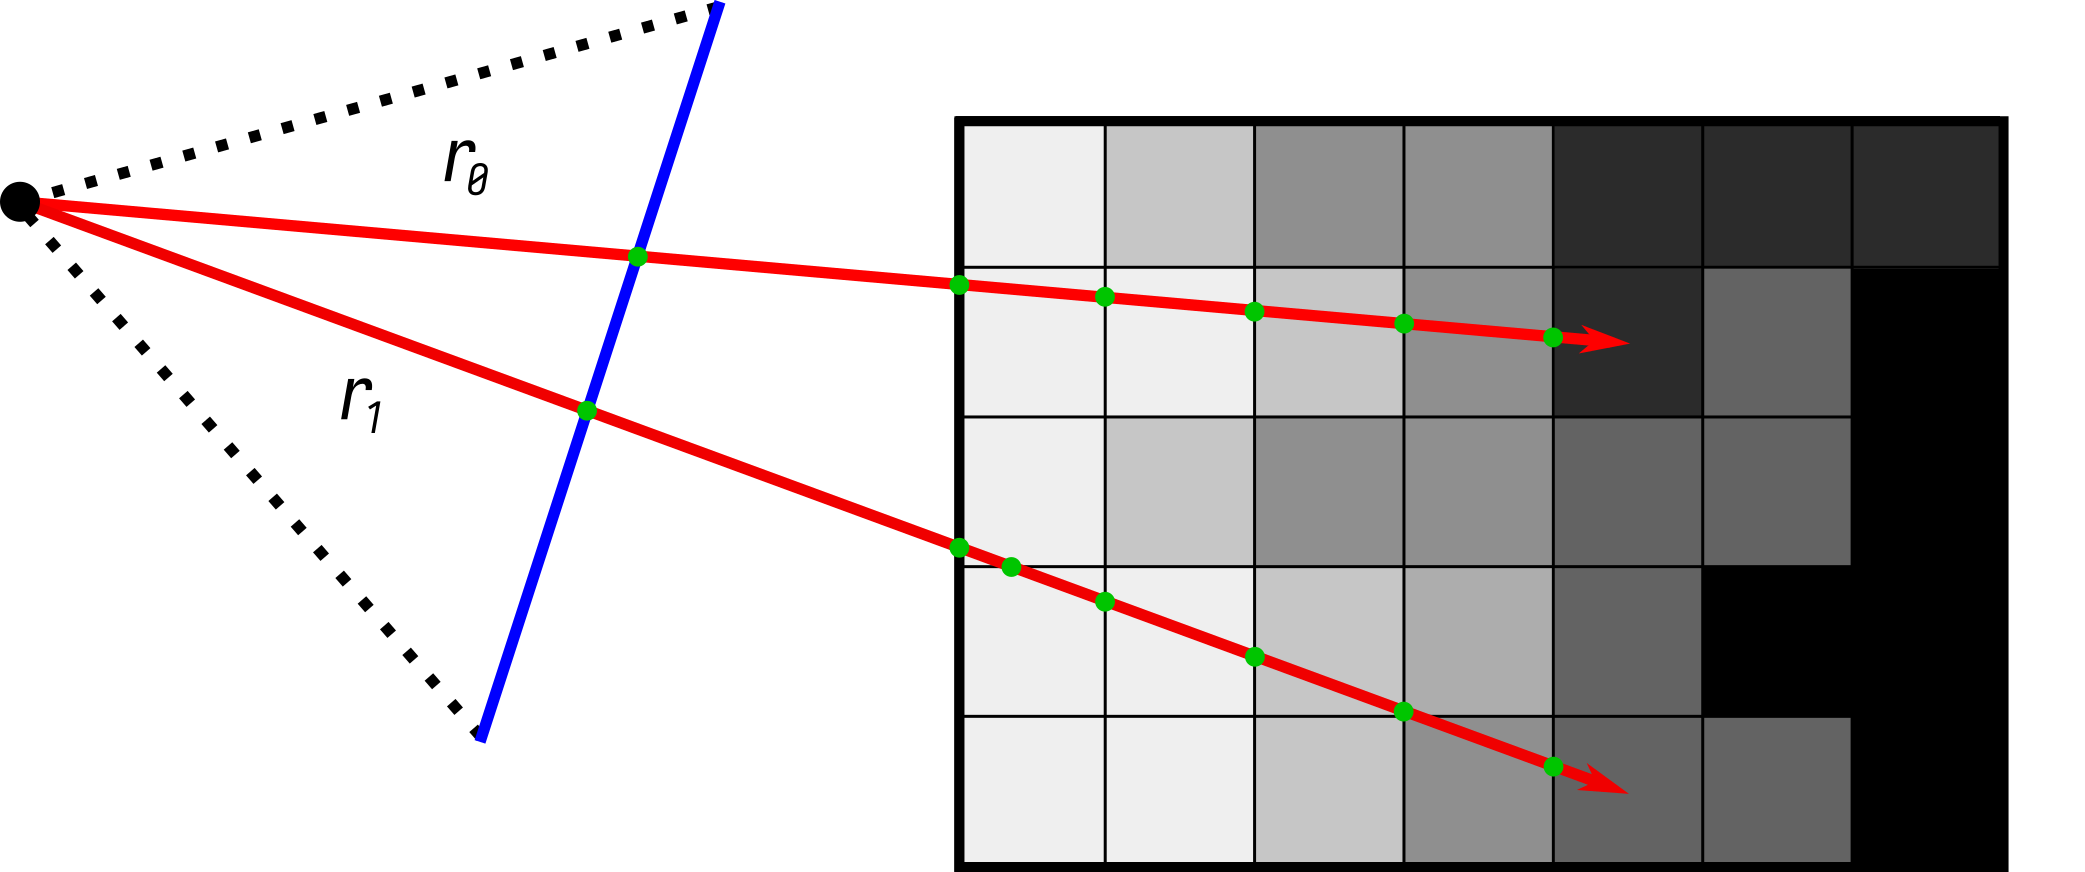
\includegraphics[width=.8\linewidth]{img/raytracing_contribution.png}
                \captionsetup{width=.8\linewidth}
                \caption{Le lancer de rayons dans une grille volumique. Les rayons (rouge) traversent les voxels de la grille aux points d'intersection (vert) en additionnant les couleurs et opacités de chacun des voxels selon une fontion de transfert définie par l'utilisateur.}
                \label{img:raytracing_contribution}
            \end{figure}

            Toutefois, bien que les méthodes basées sur le lancer de rayons soient le plus courant et le plus intuitif à comprendre, il existe quelques autres méthodes de visualisation comme celle développée par L.A. \textsc{Westover} appelée \textit{splatting}~\cite{cite_splatting}, qui vise à construire itérativement une rastérization de la grille volumique en entrée, afin de pouvoir la visualiser en temps réel. Cet algorithme permet de visualiser l'ensemble des données, mais ne permet pas d'avoir une visualisation immédiate du jeu de données, car la construction de la représentation de l'image tridimensionnelle se déroule sur plusieurs rendus successifs à l'écran.

            Ces méthodes de visualisations volumiques sont pratiques car elles permettent de visualiser l'intégralité des données du volume, sans recourir à des algorithmes de pré-traitement qui pourraient introduire des erreurs dans la reconstruction des données en isosurfaces. Toutefois, dû à leur temps de calcul beaucoup plus élevés qu'un affichage de surface, ces méthodes ne permettent pas toujours d'avoir un rendu interactif.
        }
        % }}}
        
        % hybrides {{{
        \subsection{Visualisations hybrides}
        {
            Les méthodes de visualisation surfaciques sont rapides, et demandent peu de mémoire mais sont sujettes à des erreurs dans la construction de la représentation isosurfacique d'une image tridimensionnelle. Les méthodes de visualisation volumiques offrent une visualisation exacte de l'ensemble des données contenues dans une image tridimensionnelle sans avoir besoin de pré-traitement, mais sont très coûteuses en temps et mémoire et ne permettent pas de visualisation interactive sur la majorité des stations de travail.

            Certaines méthodes de visualisation hybrides furent donc développées afin de pouvoir visualiser une image intégralement, tout en restant interactif. Ces méthodes combinent l'utilisation de géométrie qui est facile à manipuler et afficher à l'écran, avec du lancer de rayons pour visualiser l'ensemble des données présentes dans l'image. La méthode de visualisation décrite en section \ref{section:visualisation:subdomains} est un exemple d'une méthode de visualisation hybride.

            \begin{figure}[h]
                \centering
                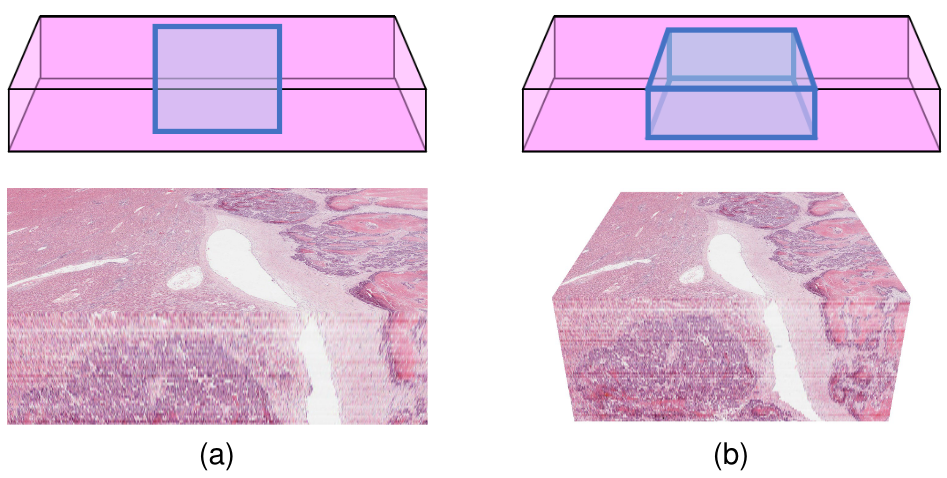
\includegraphics[width=.9\linewidth]{img/falk_et_al.png}
                \captionsetup{width=.8\linewidth}
                \caption{La différence entre une vue de scène $(a)$, et une vue par sous-volume $(b)$. Le volume originel est représenté en magenta, la zone affichée à l'écran en bleu. Depuis \textsc{Falk} \textit{et al.}~\cite{cite_3d_real_time_histopathology}.}
                \label{img:visualisation:falk}
            \end{figure}

            Plus récemment, \textsc{Falk} \textit{et al.}~\cite{cite_3d_real_time_histopathology} ont proposé une méthode de rendu hybride utilisant le lancer de rayons afin d'afficher des coupes histopathologiques à très haute résolution. Pour cela, les données sont d'abord recalées lors d'un processus hors-ligne. Ensuite, ces mêmes images sont chargées en \og{}briques~\fg qui sont stockées en forme d'octree ou d'arbres d'ondelettes par exemple. Graĉe à un retour d'experts, ils ont conclus qu'avoir une vue en sous-volume était plus intuitif que d'avoir une vue en scène, les différences de ces deux approches sont visibles en figure \ref{img:visualisation:falk}.
        }
        % }}}
    }
    % }}}

	% Partie visualisation plans de coupe {{{
	\section{Exploration volumique par plans de coupe}\label{section:visualisation:cuttingplanes}
	{
        %L'un des objectifs de ce stage est de visualiser en temps réel l'image 3D résultante d'une acquisition. Étant donné que la majorité des examens médicaux non destructifs comme l'IRM effectuent des vues en coupe d'un patient, il faut permettre aux médecins d'accéder à une méthode de visualisation qui leur est familière. Ainsi, il est nécessaire d'implémenter une méthode d'exploration du volume par plans de coupe afin de ne pas augmenter la difficulté associée à une analyse d'échantillon par un médecin, pour faciliter son diagnostic.

		L'exploration des données à l'aide de plans de coupe est une méthode simple de visualisation surfacique permettant d'explorer l'intérieur d'un volume en \og{}découpant~\fg celui-ci selon un plan donné. Cette méthode permet d'afficher l'ensemble des données présentes sur ce plan, sans afficher les éléments qui pourraient se trouver derrière. En effet, afin d'afficher les données situées derrière le plan de coupe en lui-même nécessiterait l'utilisation d'une méthode de visualisation volumique, ou d'une méthode de visualisation hybride.

		Les explorations par plans de coupe sont des outils de diagnostics rapide encore très utilisées dans la majorité des logiciels destinés aux médecins, plus fréquemment afin de pouvoir observer un tissu numérisé sous plusieurs angles différents sans avoir besoin de recourir à une nouvelle acquisition. Ainsi, une fois une image tridimensionnelle acquise il est possible de définir plusieurs plans de coupe selon le besoin du praticien et d'analyser le tissu sous un nouvel angle, ce qui peut être pratique pour certains diagnostics comme celui du cancer de la prostate par exemple.

		Nous avons implémenté une méthode d'exploration par plans de coupes alignés sur les axes dans un programme écrit en C++, avec l'aide de \textit{Qt}, \textit{OpenGL} et \textit{QGLViewer}. Ce programme permet non seulement de charger une image 3D en mémoire en utilisant les techniques présentées dans la section \ref{section:memory}, mais aussi de les visualiser une fois chargées. Pour achever une telle visualisation, nous chargerons tout d'abord les données de l'image 3D en entrée dans une texture 3D \textit{OpenGL}. Celle ci sera envoyée sur le processeur graphique, qui se chargera de l'appliquer sur un cube à l'aide de coordonnées de texture. \textit{OpenGL} possède déjà des fonctions de gestion de texture en 1, 2, ou 3 dimensions. Il nous suffit donc d'allouer un espace mémoire suffisant (réservé à l'utilisation exclusive par \textit{OpenGL}), et d'envoyer les données issues du chargement des images. Par la suite nous pouvons attribuer des coordonnées de texture à chacun des sommets du cube afin que \textit{OpenGL} puisse calculer quelle partie de la texture afficher sur un point donné du cube.

		\begin{figure}[!h]
		    \centering
		    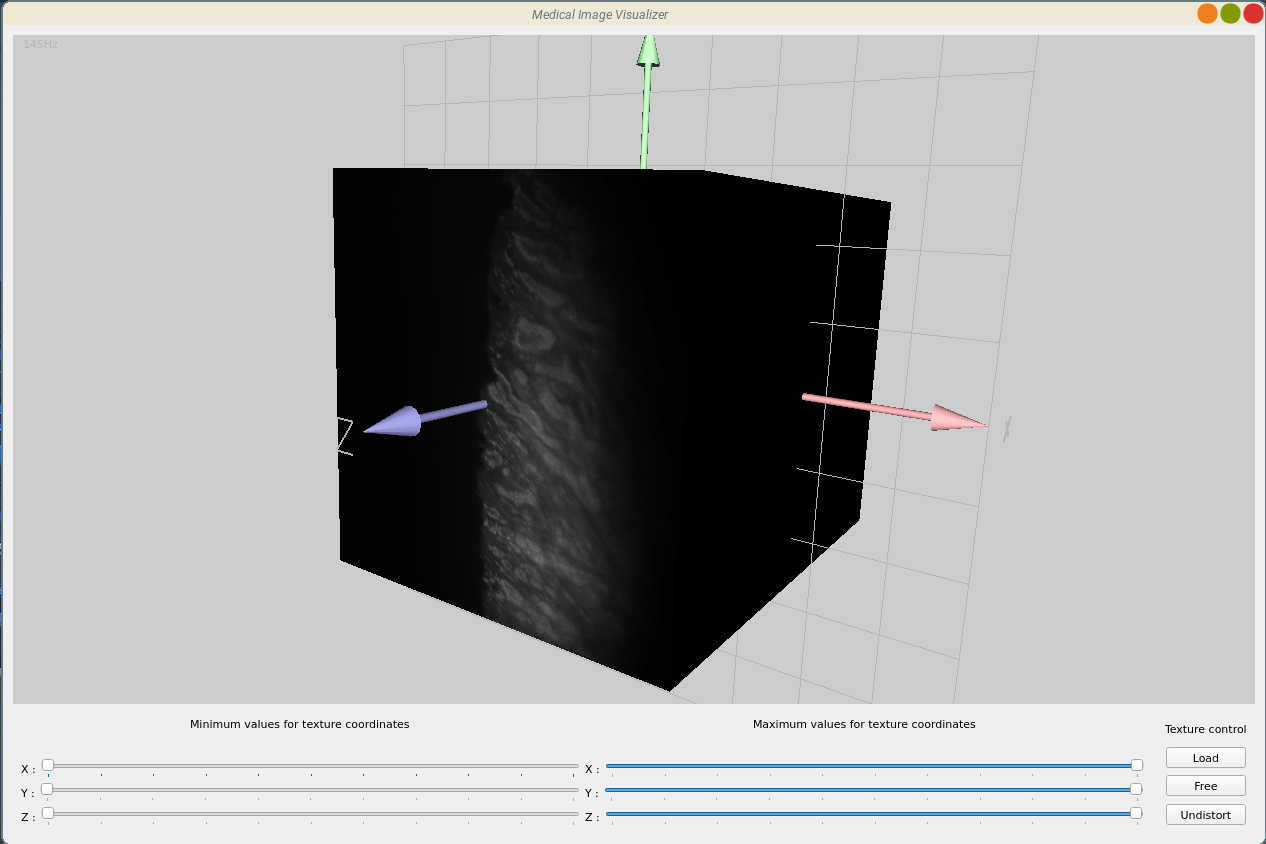
\includegraphics[width=.7\linewidth]{img/ui1.png}
		    \caption{Le programme, une fois une texture chargée.}
		    \label{img:ui_general}
		\end{figure}

        Une première amélioration qui fut implémentée à cette méthode de visualisation fut la modification de la taille du cube afin de donner une approximation visuelle du nombre d'images chargées. Une fois l'ensemble des images chargées en mémoire, la hauteur du cube est modifiée, afin d'obtenir un parallélépipède dont les côtés ont une longueur égale aux dimensions de l'image tridimensionnelle chargée. Cela permet à l'utilisateur du programme d'avoir une intuition visuelle de la quantité de données chargées, en fonction de la profondeur de la pile d'images (voir figure \ref{img:cubes}).

        \begin{figure}[!h]
            \begin{subfigure}{.49\linewidth}
                \centering
                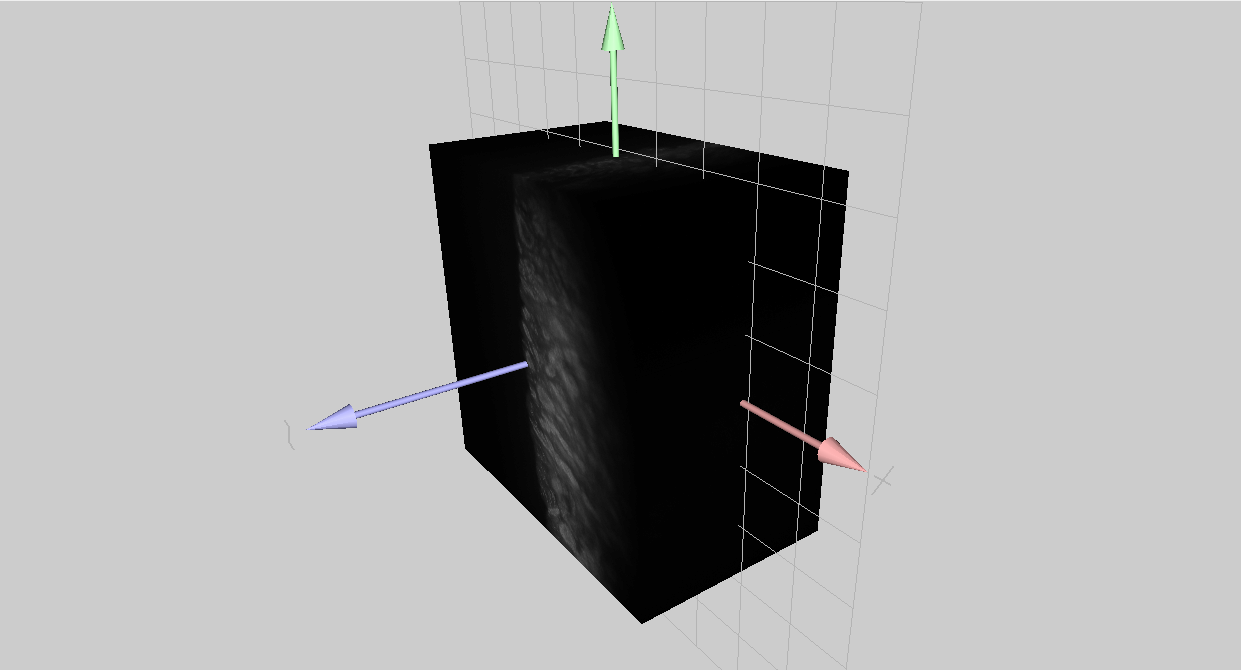
\includegraphics[width=.9\linewidth]{img/cube1.png}
                \captionsetup{width=.9\linewidth}
                \caption{Le cube permettant d'afficher la texture, mis à l'échelle pour une pile de 250 images.}
                \label{img:cube1}
            \end{subfigure}
            \hfill
            \begin{subfigure}{.49\linewidth}
                \centering
                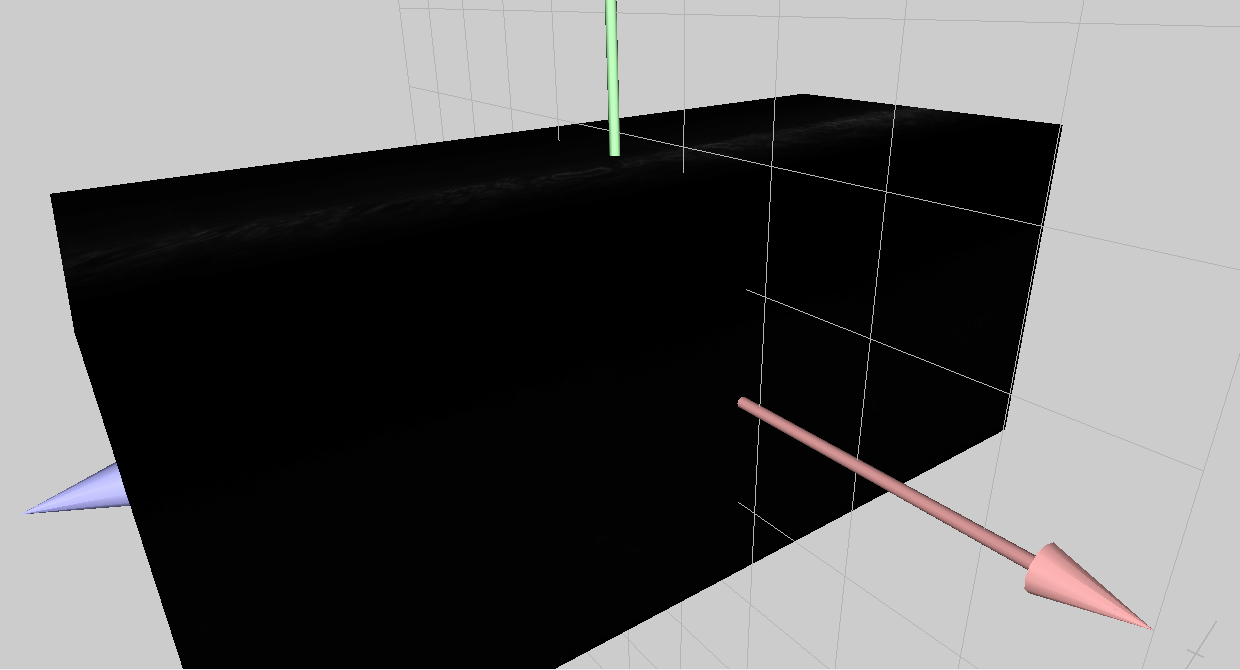
\includegraphics[width=.9\linewidth]{img/cube2.png}
                \captionsetup{width=.9\linewidth}
                \caption{Le cube permettant d'afficher la texture, mis à l'échelle pour une pile de 1000 images.}
                \label{img:cube2}
            \end{subfigure}
            \caption{Mise à l'échelle de la profondeur du cube selon le nombre d'images chargées.}
            \label{img:cubes}
        \end{figure}

		Ensuite, nous pouvons donner le contrôle à l'utilisateur de la position des plans de coupe qu'il souhaite avoir, avec des curseurs situés en bas de la fenêtre. Chacun d'entre eux est connecté\footnote{Voir annexe technique Qt} aux coordonnées X, Y, et Z de chacun des points permettent à l'utilisateur de définir les coordonnées des plans de coupe sur ces axes. Lorsque l'utilisateur décide d'appliquer un plan de coupe, il lui suffira de faire glisser le curseur à la position désirée, et le programme mettra automatiquement à jour les valeurs de position et de texture aux sommets concernés par cette modification. Par la suite, l'écran sera rafraîchi afin de refléter les changements apportés.

		\begin{figure}[!h]
            \begin{subfigure}{.49\linewidth}
                \centering
                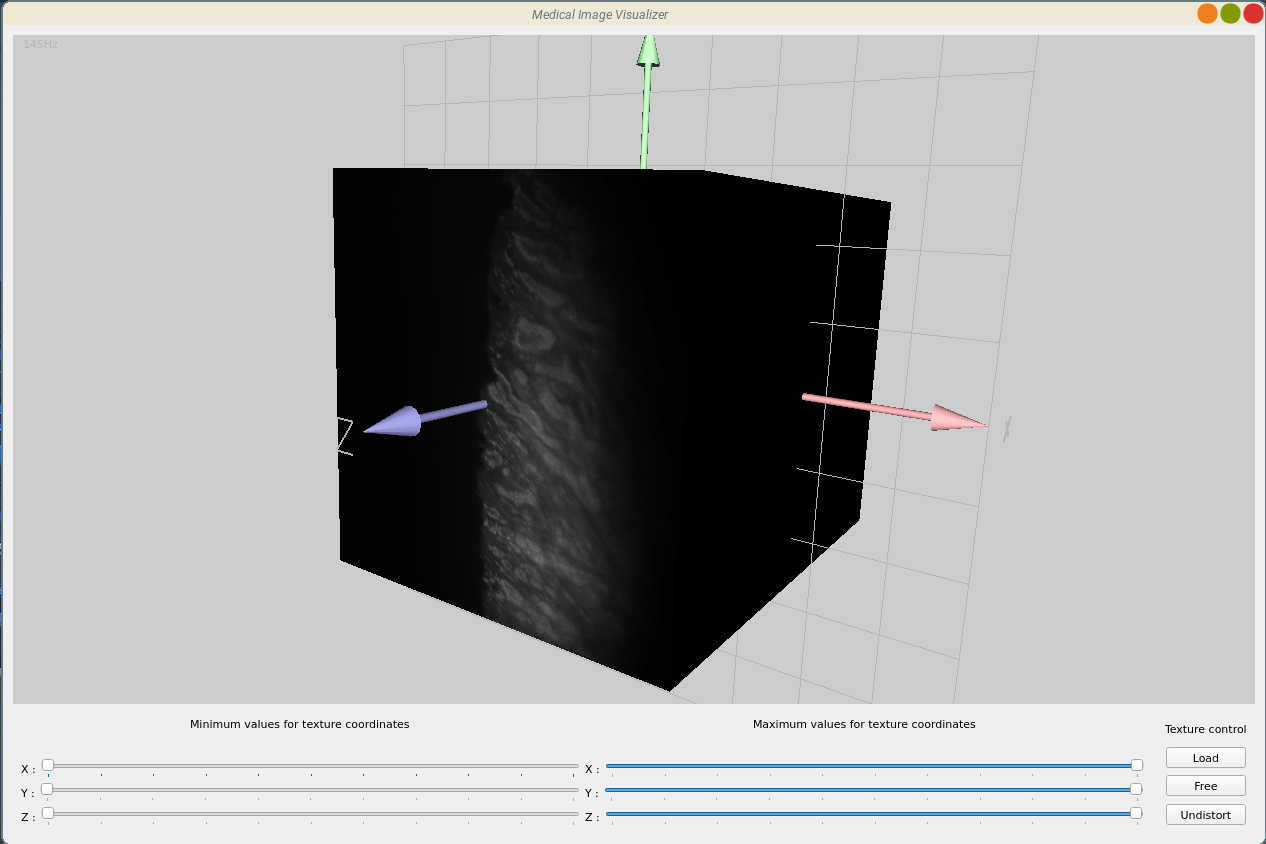
\includegraphics[width=.9\linewidth]{img/ui1.png}
                \captionsetup{width=.9\linewidth}
                \caption{Le cube, permettant un proxy entre la texture et son rendu à l'écran.}
                \label{img:ui1}
            \end{subfigure}
            \hfill
            \begin{subfigure}{.49\linewidth}
                \centering
                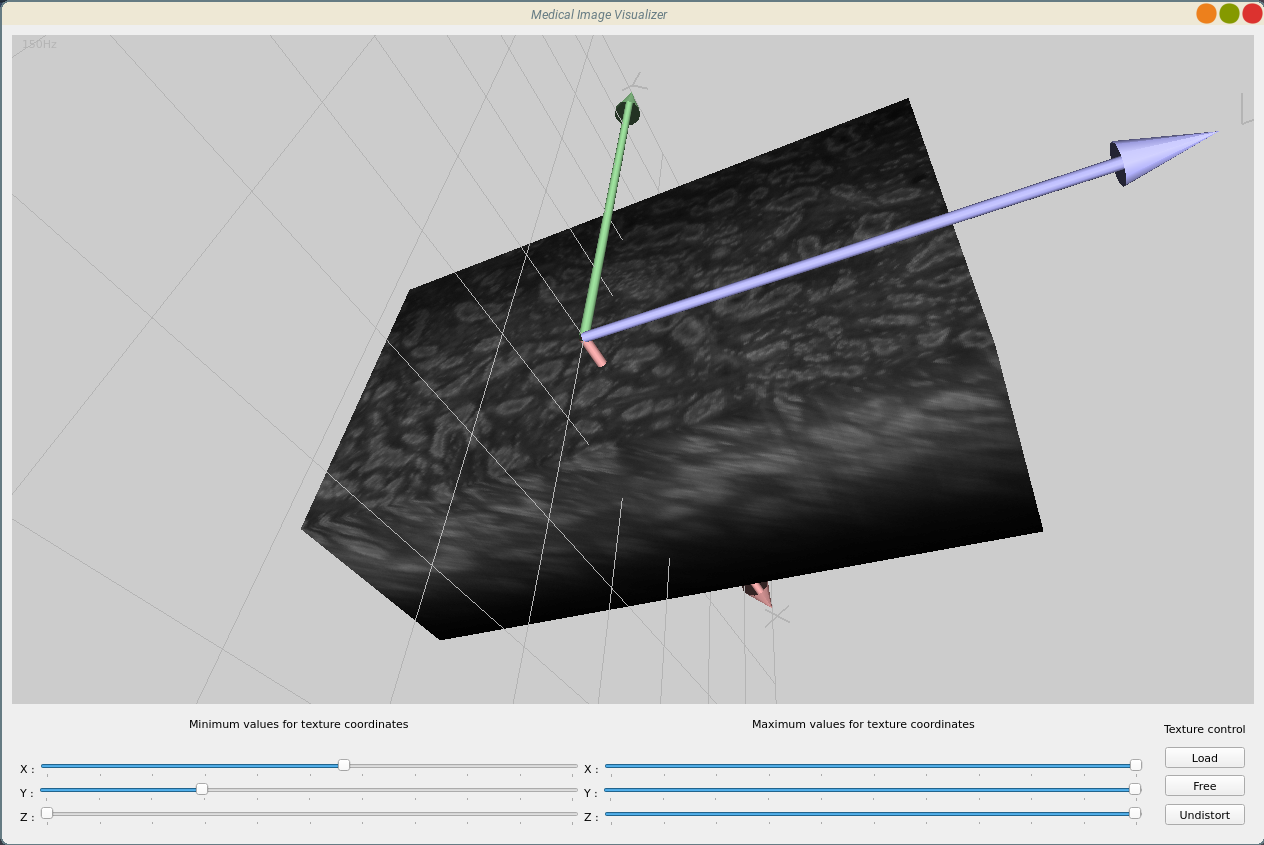
\includegraphics[width=.9\linewidth]{img/ui2.png}
                \captionsetup{width=.9\linewidth}
                \caption{Quelques plans de coupes appliqués aux images chargées.}
                \label{img:ui2}
            \end{subfigure}
            \caption{Un exemple de visualisation par plans de coupes.}
        \end{figure}

		Ainsi, nous avons présenté une technique permettant de traverser interactivement le volume sur toutes les directions, afin d'observer le tissu sous différentes facettes pour mieux comprendre sa formation interne.
	}
	% }}}

	% Partie visualisation volumique par sous-domaine {{{
	\section{Visualisation par sous-domaines}\label{section:visualisation:subdomains}
	{
	    % Plan section {{{
	    \iffalse
	    \commentaire{
	    \begin{itemize}
	        \item quel problème ? \begin{itemize}
	            \item méthode précédente cool, mais on ne peut pas voir en 3D uniquement une 'slice' de la texture
	            \item on souhaite pouvoir effectuer visu en temps réel tridimensionnel, pas plaqué sur une primitive afin de pouvoir voir la vraie forme de la grille
	        \end{itemize}
	        \item Pourquoi cette méthode de visu est dure ?~\begin{itemize}
	            \item Il faudrait avoir beaucoup de mémoire afin de l'afficher (grilles $\rightarrow$ 'n' voxels $\rightarrow$ 8*'n' points pour dessiner completement
	            \item autre méthodes de rendu volumiques $\rightarrow$ applique texture sur une primitive et recalculent selon angle de vue (beaucoup d'interpolations nécessaires pour bon résultat, artéfact visuels à certains angles ...)
	            \item permet déformation du volume en temps réel (pas trop utile pour cette application en particulier, mais pas mal !)
	        \end{itemize}
	        \item qu'est ce qu'on a apporté\begin{itemize}
	            \item méthode de visu temps réel dépendant non pas de la taille de grille, mais de la taille écran en px à rendre
	            \item permet de voir le modèle par sous-domaines, interactivement
	            \item permet de voir la vraie forme de la donnée dans la grille
	            \item permet de déformer le modèle si besoin (bonus !)
	        \end{itemize}
	    \end{itemize}
	    }
	    \fi
	    % }}}

		% Intro {{{
		Une exploration par plans de coupe est utile, et permet une visualisation interactive de la texture représentant la donnée acquise par le microscope. Toutefois, le but du projet étant l'analyse de la forme tridimensionnelle des glandes de la prostate, il est nécessaire de posséder une méthode de visualisation volumique interactive permettant de n'afficher qu'une certaine plage de données, correspondant par exemple à une zone d'intérêt dans l'échantillon. Cela nous permettrait d'obtenir une visualisation interactive des données sans avoir besoin d'utiliser de géométrie intermédiaire à la visualisation.

		Ainsi, en plus de la visualisation en plans de coupe, nous proposons une visualisation de grilles de voxels par sous-domaines\definition{Plage de valeurs représentant un type particulier de données}. Cette méthode permet de visualiser uniquement les informations que l'utilisateur souhaiterait examiner. Par exemple, si l'on définit un sous-domaine représentant la membrane d'une glande dans un échantillon de prostate, nous pourrions afficher uniquement les données faisant parties de leur sous-ensemble dans l'échantillon entier, et ainsi représenter à l'écran la morphologie de celles-ci. Les travaux effectués sur la méthode pendant cette partie du stage furent intégrés à un article soumis à la conférence IEEE VIS 2020\footnote{\url{http://ieeevis.org/year/2020/welcome}}, co-écrit par Mme \textsc{Faraj} (Université de Montpellier), Jean-Marc \textsc{Thiery}, Tamy \textsc{Boubekeur} (tous deux Télécom Paris), Brian \textsc{Summa} (Université de Tulane).\par
		% }}}

		% Présentation méthode {{{
		\subsection{Présentation de la méthode}
		{
		    Comme expliqué précédemment, il est nécessaire de proposer une méthode de rendu volumique d'une grille de voxels, ne se basant pas sur la projection d'une texture sur une primitive comme l'est l'exploration par plans de coupe. En effet, même si ces techniques sont pratiques car elles permettent de traverser un espace tridimensionnel, elles n'offrent aucune possibilité de transparence. Il nous faut donc développer un autre type de méthode de visualisation.

			Cette méthode de visualisation de grilles de voxels est une visualisation hybride, qui fut originellement développée afin d'analyser l'effet de l'exposition aux émissions électromagnétiques sur le corps humain. La méthode utilise deux composants afin de rendre à l'écran la grille de voxels (définition disponible en section \ref{section:voxelgrid}). En premier lieu, il faut charger une grille de voxels. Il faut ensuite charger un maillage tétraédrique, représentant une surface englobant l'objet analysé. Ce maillage permet de paver l'espace intérieur à la grille de voxels. Ensuite, des coordonnées de texture sont calculées pour chacun des sommets du maillage tétraédrique, ainsi que certaines données constantes à chacun des tétraèdres (comme le voisinnage direct de chacun d'entre eux par exemple). L'ensemble des données est ensuite envoyé sur le processeur graphique, où l'on pourra faire un rendu à l'écran de la grille par la suite.

			Une fois les étapes de pré-traitement réalisées, le programme effectue une boucle de rendu afin d'afficher le maillage à l'écran, comme le feraient la grande majorité des programmes de visualisation volumique traditionnels. La différence est qu'une fois que le rendu du maillage est calculé après l'étape de rastérisation\definition{Processus de projeter une primitive 3D sur un écran 2D. Voir annexe technique \textit{OpenGL}}, une étape de lancer de rayons\definition{Processus de recherche d'intersections le long d'un rayon. Voir annexe technique \textit{OpenGL}}, aussi appelé \textit{ray-casting} est effectuée à l'intérieur des tétraèdres du maillage afin de parcourir la grille de voxels, et de trouver le premier voxel sur le chemin du rayon incident qui représente une information. Si une intersection n'est pas trouvée dans le système de coordonnés barycentriques du tétraèdre courant, le rayon va visiter les tétraèdres voisins afin de trouver une information à afficher. À partir du rayon incident, nous pouvons également extraire la normale en ce point, ainsi que la couleur qu'il devrait prendre, afin de simuler un voxel sur l'écran de l'utilisateur. Vous pourrez trouver un exemple schématique de cette opération en figure \ref{img:kpf_principle}.

			\begin{figure}[h]
			    \centering
			    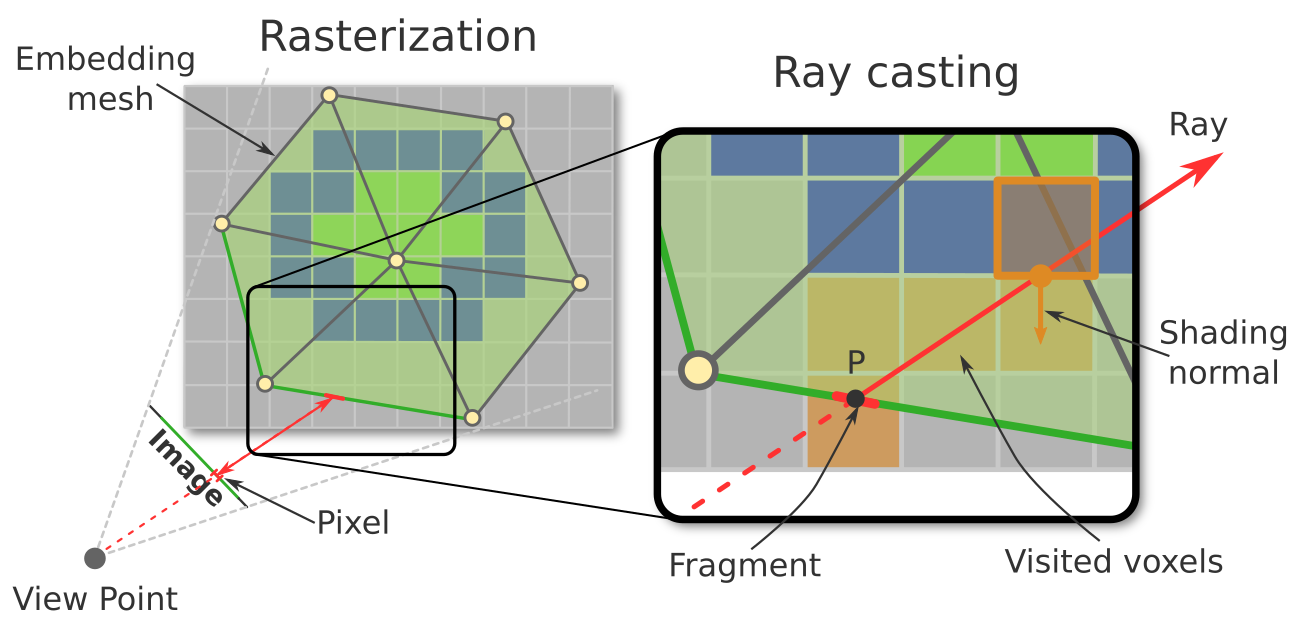
\includegraphics[width=.8\linewidth]{img/raytracing_grid_principle.png}
			    \caption{Lancer de rayon dans la grille, à partir de la rastérisation du maillage englobant}
			    \label{img:kpf_principle}
			\end{figure}

			La rastérisation originelle du maillage tétraédrique permet de trouver le point d'entrée $P$ dans la grille de voxels comme illustré en figure \ref{img:kpf_principle}. C'est à partir de ce point que le lancer de rayons va prendre place dans le maillage.

			En plus de la visualisation par sous-domaines, il est possible d'ajouter un plan de coupe afin de ne rendre les tétraèdres non occultés celui-ci, pour pouvoir traverser le modèle de façon naturelle. Cette opération peut être réalisée en ne prenant que les fragments rastérisés des tétraèdres non entièrement cachés par le plan de coupe, afin de trouver le point $P$ d'entrée dans la grille.
			
			Étant donné que le processus de lancer de rayon effectue une vérification de chaque voxel le long du rayon, il est trivial de catégoriser ce qui est considéré comme une information valide, par rapport à ceux qui n'en sont pas. Il suffit d'utiliser en plus de la grille un tableau contenant un indice de visibilité par sous-domaine, ou bien une fontion de transfert pour cette grille. Grâce à cela, il est possible de ne rendre à l'écran que certains sous-domaines afin de voir une image tridimensionnelle partielle de la grille.

			Cette méthode permet de visualiser des grilles de voxels de plusieurs millions d'éléments (comme \textit{Louis} avec 249 millions de voxels) à plus de 100 rafraîchissements par seconde, et à plus de 60 rafraîchissements par seconde avec des plans de coupe !

			Grâce à cette méthode, nous pouvons afficher interactivement des grilles de voxels de très haute résolution, où la complexité dépend de la taille de l'écran en pixels, et la seule limite imposée est dictée par la taille de la mémoire disponible sur la carte graphique. En figure \ref{img:hands}, vous trouverez un exemple de visualisation en sous-domaines.
			
			\begin{figure}[!h]
			    \centering
    			\begin{subfigure}{.49\linewidth}
    			    \centering
    			    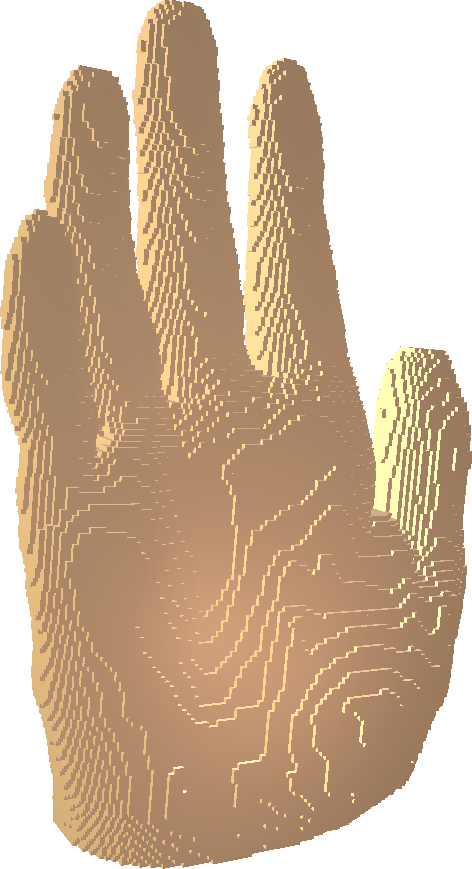
\includegraphics[width=.6\linewidth]{img/hand.png}
    			    \label{img:hand}
			    \end{subfigure}
			    \hfill
    			\begin{subfigure}{.49\linewidth}
    			    \centering
    			    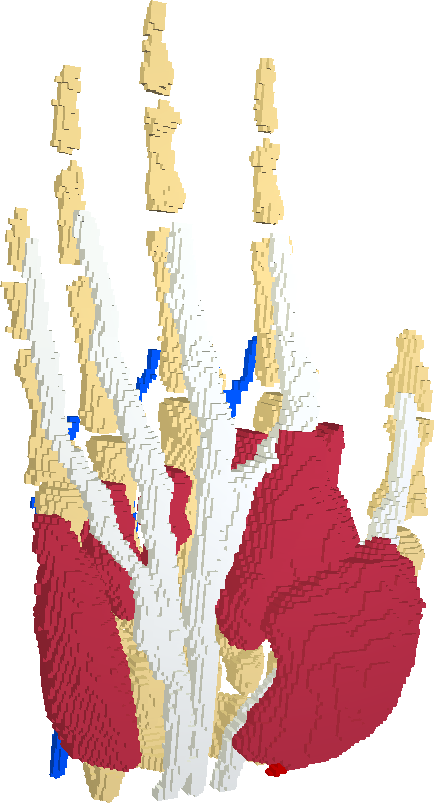
\includegraphics[width=.6\linewidth]{img/hand_less.png}
    			    \label{img:hand_less}
			    \end{subfigure}
			    \caption{Un modèle de main, visualisé entièrement à gauche, et avec uniquement certains sous-domaines à droite (tissus osseux, tendons avant/arrières et muscles).}
			    \label{img:hands}
			\end{figure}
		}
		% }}}

		% Travail effectué {{{
		\subsection{Travail effectué}
		{
			La méthode de rendu volumétrique fut premièrement implémentée par Mme \textsc{Faraj} il y a de cela quelques années. Les contributions apportées pendant cette période de stage furent triples : tout d'abord, une mise à jour du code fut effectuée afin que le logiciel soit plus stable. Ensuite, la méthode de chargement des grilles en mémoire fut adaptée afin d'être capables de charger des grilles plus grandes en mémoire. Enfin, le logiciel fut testé sur plusieurs jeux de données, à plusieurs résolutions différentes et dans plusieurs cas différents.

			La première implémentation de la méthode ayant été écrite dans des versions anciennes de \textit{boost}\footnote{Bibliothèque utilitaire écrite en C++, permettant de gérer beaucoup d'aspects d'un programme sur plusieurs plateformes.} et \textit{CGAL}\footnote{Bibliothèque de traitement géométrique écrite en C++.}, la première tâche effectuée avant même de commencer à travailler sur le programme en lui même fut de retrouver et de recompiler les versions nécessaires des bibliothèques, toutes deux ayant subis de nombreux changements depuis leur utilisation antérieure.

			Une fois ces problèmes d'incompatibilité inter-bibliothèques résolus, la prochaine tâche fut de régler certains problèmes liés aux \textit{shaders}\definition{Programme décrivant comment générer une image rendue à l'écran à partir de primitives} du programme. En effet, ceux ci furent écrits lorsque \textit{OpenGL} était encore peu développé, et nécessitaient un peu de travail afin de fonctionner efficacement sur de nouvelles architectures de cartes graphiques. Une étude approfondie de la méthode a donc du être réalisée afin de mieux comprendre non seulement la méthode en elle-même, mais aussi le code l'accompagnant.

			Dans la première version de la méthode, le choix fut pris d'envoyer sur la carte graphique la grille de voxels avec une couleur préattribuée pour chaque voxel, sous la forme d'un vecteur quadridimensionnel contenant les composantes rouge, verte, bleue, et de transparence. En effet, il est nécessaire d'avoir une couleur par voxel lors de la visualisation, afin de déterminer à l'oeil nu les sous-domaines présents dans une image. Or, la grille étant pré-segmentée en sous-domaines, il est possible de décorréler les informations de couleur des voxels de la grille en elle-même. En effet, les valeurs représentant ces sous-domaines étant des nombres entiers non nuls, il nous est possible de les utiliser pour adresser un tableau de couleurs précalculé. Ainsi, nous pouvons récupérer l'information nécessaire pour afficher une couleur uniquement au moment où elle est nécessaire, allégeant la taille mémoire utilisée par la grille. De cette façon, nous pouvons augmenter la taille maximale des grilles chargées sur la carte graphique, en ne stockant qu'un atlas de couleurs à ses côtés.

			Une fois cette modification implémentée, un problème d'implémentation est apparu : l'opération de chargement calculait les dimensions du tableau à allouer pour stocker la grille en mémoire sur 32 bits. Nous ne pouvions donc charger que des images jusqu'à 4 giga octets en mémoire. Cela ne posait pas de problème avant, mais maintenant que nous avions des jeux de données plus grands, il fallait réparer cette mauvaise implémentation en effectuant le calcul de taille ainsi que l'allocation mémoire sur 64 bits.

			Afin de tester les performances de notre application sur des données massives, un algorithme de suréchantillonage fut développé afin de créer plusieurs versions de nos grilles de tests pour montrer la résilience du programme à la taille des grilles chargées.
			Les images étant segmentées, le suréchantillonnage se devait d'être fait avec de l'interpolation au plus proche voisin, afin de ne pas perdre l'information contenue dans la grille originelle tout en augmentant la taille des fichiers de grilles en eux-même. Ainsi, à partir d'un modèle du Visible Human de 400Mo pour une grille de 400 millions de voxels, nous avons pu obtenir au final un modèle de 6.5Go, équivalent à une grille de 6.5 milliards de voxels. Nous avons donc pu tester les performances du programme sur plusieurs tailles de grilles.

			\subsubsection{Méthodologie de tests}
			{
                Afin d'effectuer des tests permettant de jauger la performance de la méthode, nous avons mis en place une méthodologie consistant de trois types d'évaluation contenant chacune trois modalités d'interactions, le tout sur deux résolutions et sur plusieurs modèles. En effet, la complexité de cette méthode est définie par le nombre de pixels à rendre à l'écran, et non pas selon la taille de la grille ou du maillage en entrée. Nos tests utilisent donc deux résolutions, $677~\times~796$ et $1347~\times~807$. Ces deux résolutions furent choisies car elles permettent de voir comment augmente la complexité quand le nombre de pixels double ($677~\times~796~=~538892$ pixels, et $1347~\times~807~=~1087029$ pixels, ou environ deux fois plus de pixels).

                Les trois types d'évaluations furent des modalités de \og{}recouvrement~\fg de l'écran par le maillage tétraédrique. Nous définissons la notion de \og{}recouvrement~\fg ici comme la proportion de pixels à l'écran qui doivent afficher une information autre que la couleur de fond. En effet, étant donné que le processus de lancer de rayons n'est initié que si un tétraèdre est rastérizé sur un pixel de l'écran, la partie de l'écran que recouvre le maillage doit influer grandement sur les performances du programme. Ainsi, les trois types d'evaluation furent les suivantes :\begin{itemize}
                    \item le modèle est entièrement visible à l'écran, et donc ne recouvre qu'une petite partie de l'écran;
                    \item le modèle est proche de l'écran, et recouvre entre un tiers et la moitié de l'écran;
                    \item le modèle est très proche de l'écran, pour un examen en détail de ses caractéristiques. Il recouvre presque entièrement l'écran.
                \end{itemize}

			    Et enfin, nous avions trois modalités d'interactions avec le modèle. La première modalité consiste à faire tourner le modèle à grande vitesse indéfiniment, afin de pouvoir tester les limites de la méthode lors d'une utilisation dans un environnement très changeant. Nous avons ensuite ajoutés deux modalités de plus, à cause d'un comportement que nous avons observé sur les modèles à forme humaine. Dû au fait que les modèles furent acquis à partir de coupes cadavériques, le nombre de voxels à traverser était plus grand lorsque l'on regardait un modèle de face, plutôt que de dos, rajoutant de la complexité à l'étape de lancer de rayon comme peut etre vu en figure \ref{img:voxel_grid_traversal_difference}. Ainsi, nous avons rajouté une modalité de manipulation manuelle précise (afin de simuler une inspection détaillée) faisant face au modèle, et une faisant dos au modèle.

			    \begin{figure}[h]
			        \centering
			        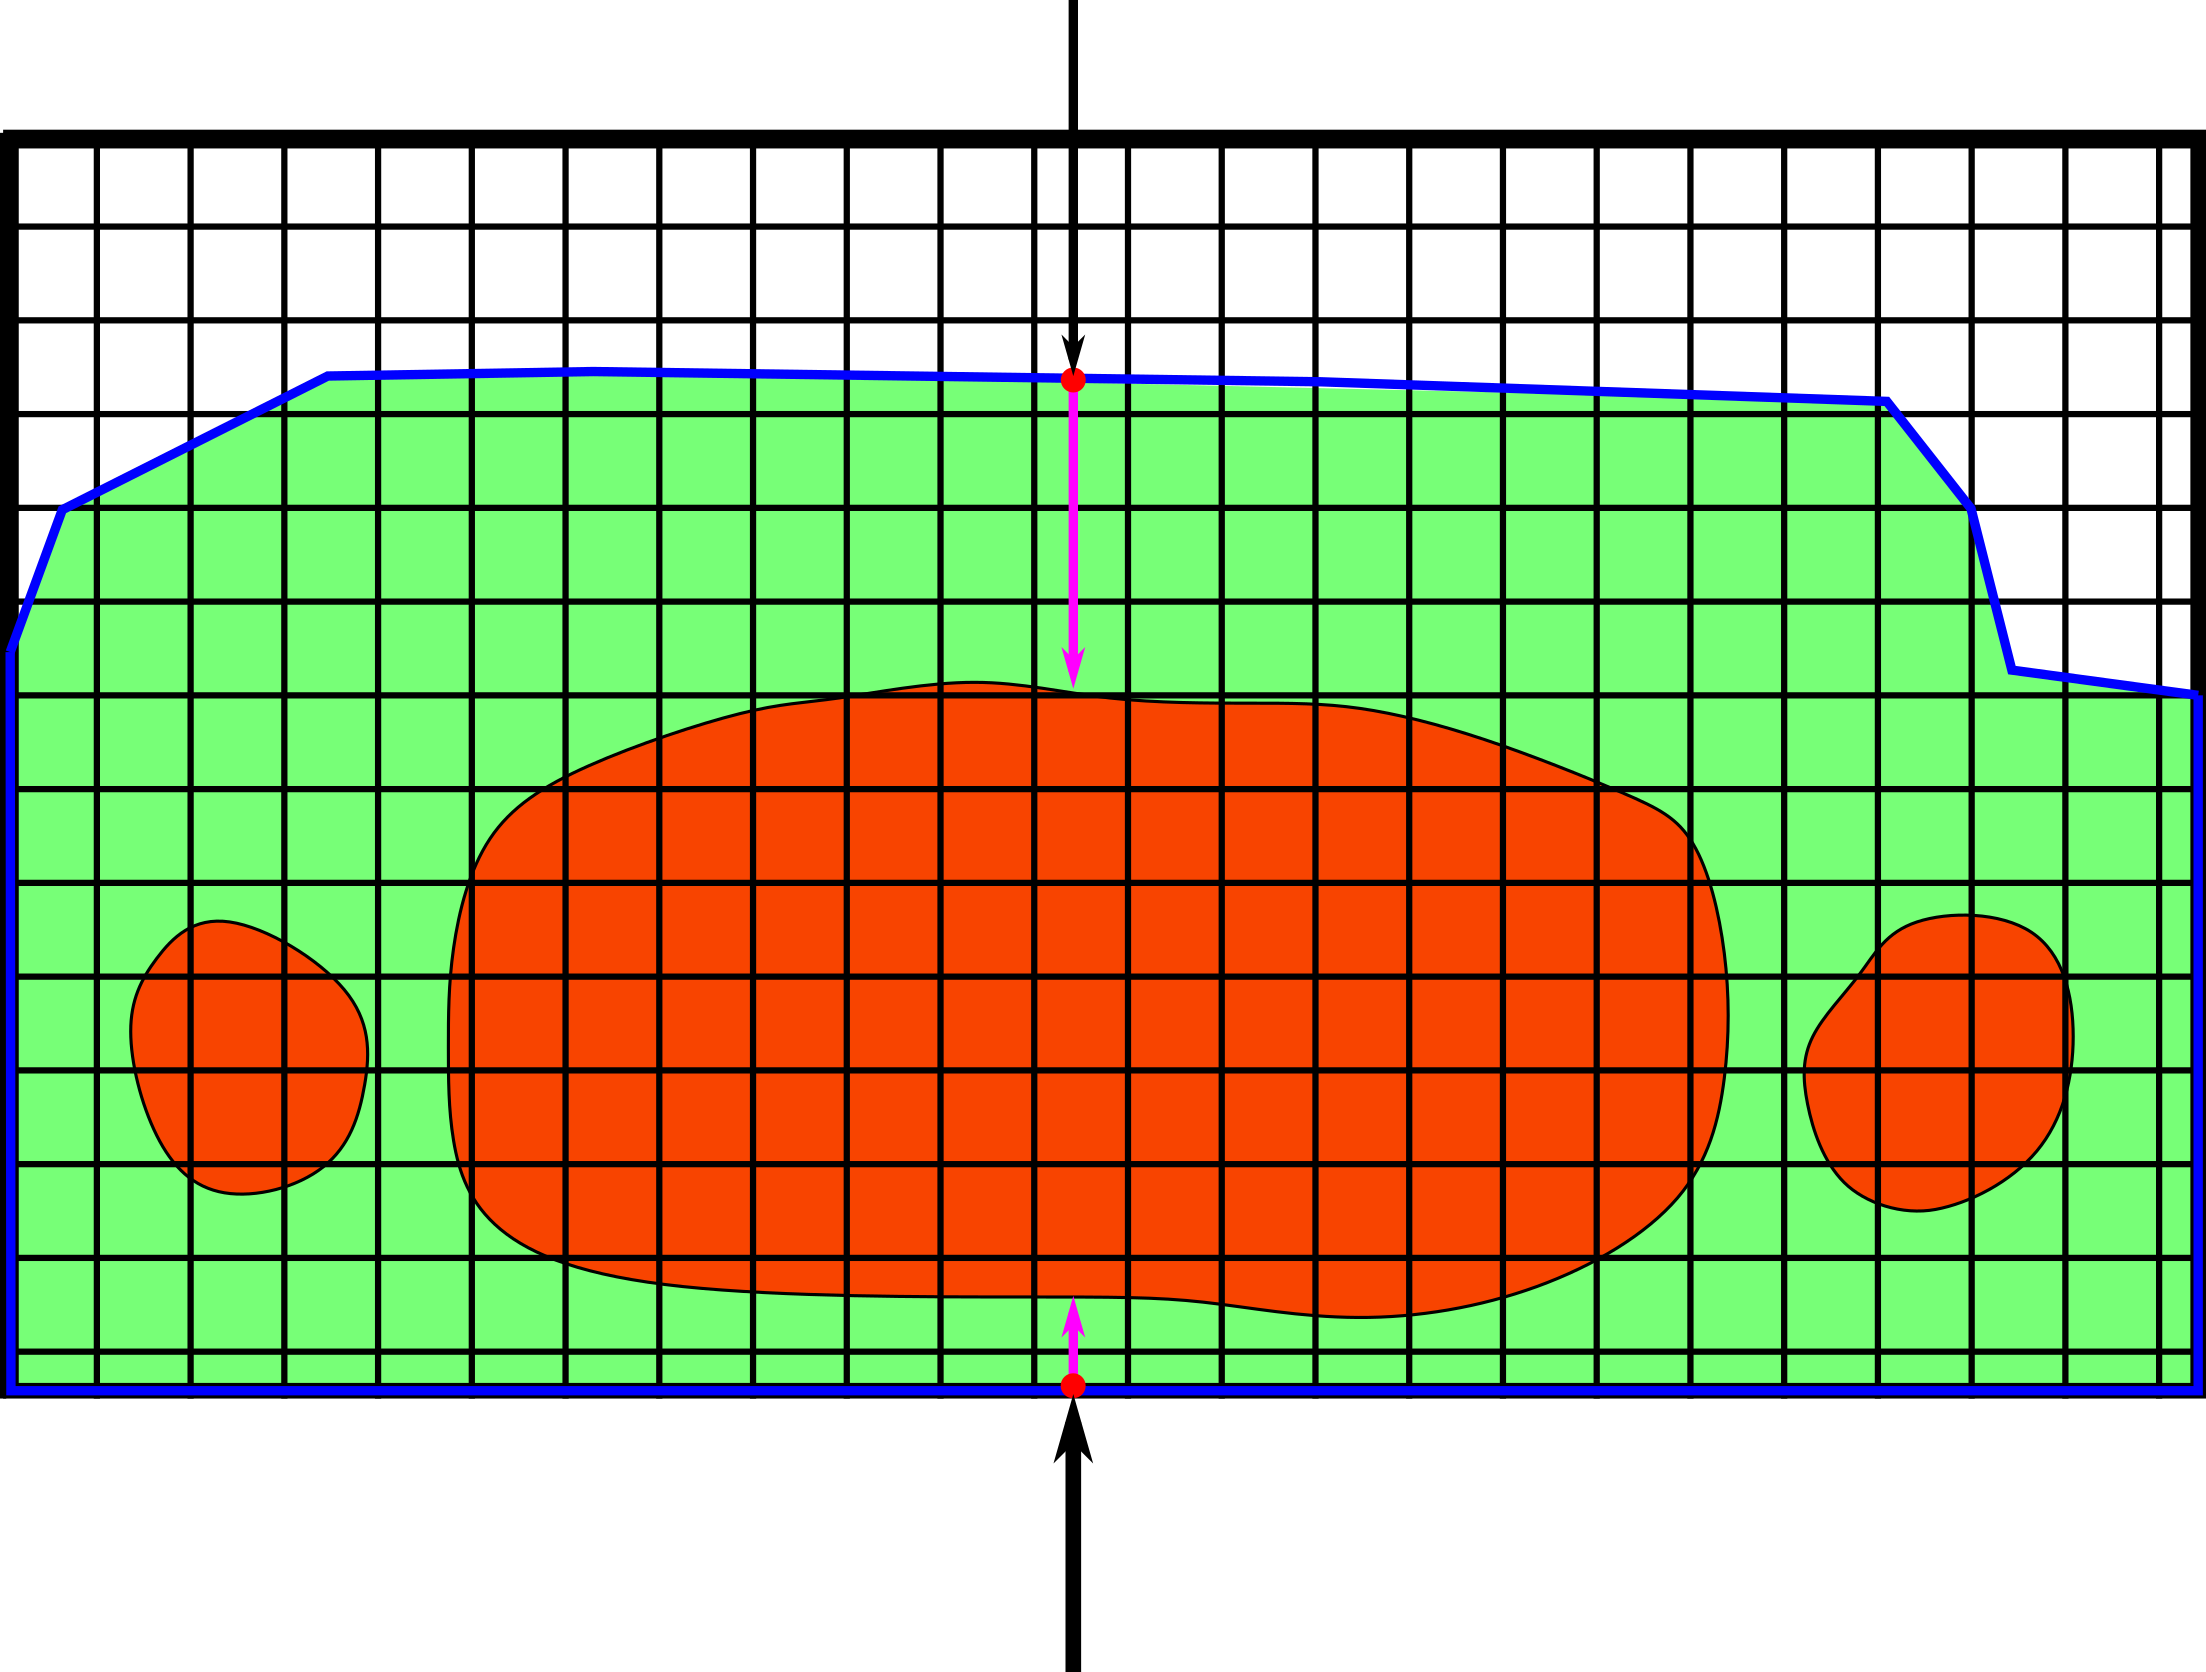
\includegraphics[width=.8\linewidth]{img/voxel_raycast_difference.png}
			        \caption{Différence de profondeur de traversée dans la grille de voxels à partir du maillage englobant (bleu). Les rayons (magenta) lancés depuis l'arrière peuvent être calculés plus rapidement que ceux de l'avant, nécessitant une exploration plus profonde dans les tétraèdres (non représentés ici pour plus de clarté)}
			        \label{img:voxel_grid_traversal_difference}
			    \end{figure}
			    
			    Le tableau complet des résultats est disponible en annexe, il détaille chacun des résultats sur chacun des modèles testés, et contient une description de la combinaison matérielle et logicielle qui a permis d'obtenir ces résultats. La grille représentant \textit{Visible Human} fut testée à deux résolutions différentes : une première fois à 800 millions de voxels (suréchantillonnée depuis la grille source, noté '0' dans le tableau des résultats) et une seconde fois à 6.5 milliards de voxels (suréchantillonné une fois de plus sur tous les axes, noté '1' dans le tableau des résultats). Il est important de noter que les deux versions de \textit{Visible Human} furent visualisés sous deux différents maillages : un maillage basse résolution (\textit{LR}), et un maillage haute résolution (\textit{HR}). \textit{Visible Human}, ainsi que la grille de voxels nommée '\textit{Louis}' furent les sujets de tests de performance avec l'utilisation des plans de coupe.
			    
			    La méthode développée permet d'afficher interactivement des modèles de plusieurs millions de voxels. Par exemple, si l'on prend le modèle \textit{Eartha}, composé de plus de 224 millions de voxels, peut être affichée et manipulée à plus de 100 rafraîchissements par seconde, dans le cas le plus intensif (où le modèle recouvre la quasi-totalité de l'écran). Sous conditions moins extrêmes, il est possible de faire afficher ce modèle à plus de 250 rafraîchissements par seconde.
			}
		}
		% }}}

		Cette méthode de visualisation par sous-domaines est rapide, efficace et permet une exploration interactive de la grille de voxels chargée en mémoire. Bien sûr, il serait possible d'ajuster cette méthode pour fonctionner avec les autres travaux réalisés au cours de ce stage, notamment pour fonctionner directement avec des images non-segmentées. Une première idée serait de pouvoir charger un modèle à multi-résolution hiérarchique en mémoire, et charger uniquement la partie que l'utilisateur souhaiterait visualiser. Pour cela, il existe plusieurs types de fichiers pouvant supporter le stockage d'images à résolution hiérarchique, comme les fichiers HDF5\footnote{\url{https://www.hdfgroup.org/solutions/hdf5/}}, permettant un stockage hiérarchique de plusieurs jeux de données, afin de pouvoir charger uniquement le modèle à la résolution que nous avons besoin, et de charger des parties détaillées à la demande de l'utilisateur.
	}
	% }}}

}

% VIM modeline : do not touch !
% vim: set spell spelllang=fr :
